% !TEX TS-program = pdflatex
% !TEX encoding = UTF-8 Unicode

% This is a simple template for a LaTeX document using the "article" class.
% See "book", "report", "letter" for other types of document.

\documentclass[12pt]{report} % use larger type; default would be 10pt

\usepackage[utf8]{inputenc} % set input encoding (not needed with XeLaTeX)

%%% Examples of Article customizations
% These packages are optional, depending whether you want the features they provide.
% See the LaTeX Companion or other references for full information.

%%% PAGE DIMENSIONS
\usepackage{geometry} % to change the page dimensions
\geometry{letterpaper} % or letterpaper (US) or a5paper or....
% \geometry{margin=2in} % for example, change the margins to 2 inches all round
% \geometry{landscape} % set up the page for landscape
%   read geometry.pdf for detailed page layout information

\usepackage{graphicx} % support the \includegraphics command and options

\usepackage[parfill]{parskip} % Activate to begin paragraphs with an empty line rather than an indent
\usepackage{cancel}
\usepackage{relsize}
%%% PACKAGES
\usepackage{booktabs} % for much better looking tables
\usepackage{array} % for better arrays (eg matrices) in maths
\usepackage{paralist} % very flexible & customisable lists (eg. enumerate/itemize, etc.)
\usepackage{verbatim} % adds environment for commenting out blocks of text & for better verbatim
\usepackage{subfig} % make it possible to include more than one captioned figure/table in a single float
\usepackage{mathtools}
\usepackage{amsmath}
\usepackage{caption}
\captionsetup{
    width=0.9\linewidth, % width of caption is 90% of current textwidth
    labelfont=bf,        % the label, e.g. figure 12, is bold
    font=small,          % the whole caption text (label + content) is small
    format=hang,         % no caption text under the label
}
% These packages are all incorporated in the memoir class to one degree or another...

%%% HEADERS & FOOTERS
\usepackage{fancyhdr} % This should be set AFTER setting up the page geometry
\pagestyle{fancy} % options: empty , plain , fancy
\renewcommand{\headrulewidth}{0pt} % customise the layout...
\lhead{}\chead{}\rhead{}
\lfoot{}\cfoot{\thepage}\rfoot{}

%%% SECTION TITLE APPEARANCE
\usepackage{sectsty}
\allsectionsfont{\sffamily\mdseries\upshape} % (See the fntguide.pdf for font help)
% (This matches ConTeXt defaults)

%%% ToC (table of contents) APPEARANCE
\usepackage[nottoc,notlof,notlot]{tocbibind} % Put the bibliography in the ToC
\usepackage[titles,subfigure]{tocloft} % Alter the style of the Table of Contents
\renewcommand{\cftsecfont}{\rmfamily\mdseries\upshape}
\renewcommand{\cftsecpagefont}{\rmfamily\mdseries\upshape} % No bold!

%%% END Article customizations

%%% The "real" document content comes below...

\title{Introduction to Electric Circuits}
\author{Darby Hewitt, PhD}
%\date{} % Activate to display a given date or no date (if empty),
         % otherwise the current date is printed 

\begin{document}
\maketitle

\chapter{Welcome!}
\label{chap:welcome}
Hello folks, and welcome to the exciting world of electric circuits! In this course, you will learn 90\% of everything you would need to be a pro in this exciting field.\footnote{I made this statistic up, but I think it's true.} And if you are doubting me in my description of this course and its subject matter as ``exciting'', let me borrow the words of Jesus Himself and say, ``stop doubting and believe\footnote{John 20:27}''. Yes, I \textit{did} just go there. 
\par
First things first---you will likely get overwhelmed in this course by all of the material we cover. However, I promise you, it's all connected, and I think it helps to think about just \textit{how} everything in electric circuits and electronics is connected before we dive in.
\par
\textbf{When you feel confused, remember that all circuits you will encounter in life fit into just two categories:}
\begin{itemize} 
\item \textbf{circuits that deliver power to something}
\item \textbf{circuits that condition signals (i.e., manipulate information)}
\end{itemize}

Some circuits fit neatly into one or the other of these categories while some circuits fit into both, but no circuits fit into any other category, broadly speaking. The Venn diagram of Figure \ref{categoriesVennDiagram} illustrates the simplicity of these circuit categories.
\begin{figure}[h]
\centering
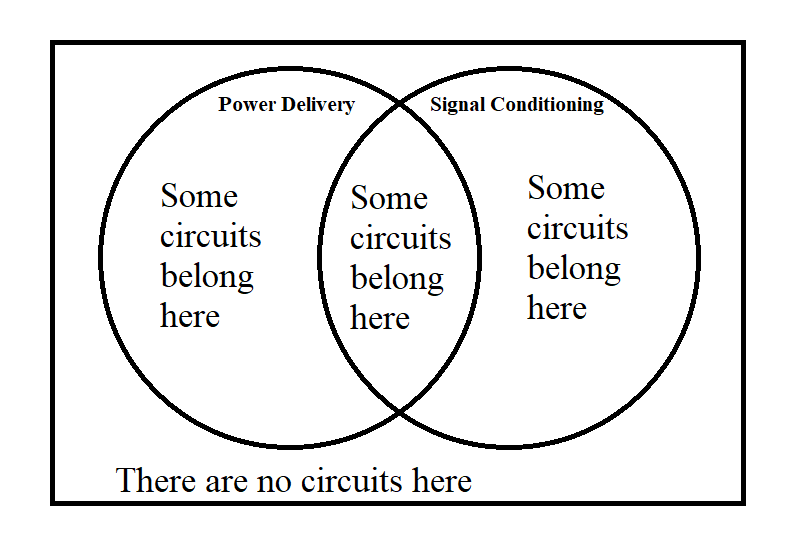
\includegraphics[width=15cm]{figures/vennDiag.png}
\caption{This comprehensive Venn diagram includes all the categories of circuits.}
\label{categoriesVennDiagram}
\end{figure}
\par
Because the categories of circuits are so few, linking the concepts in this course together should not be difficult. When you wonder why we are studying a specific topic, just think about the circuit categories; you will likely be able to connect the material in question to either powering devices or to conditioning signals. Furthermore, the first half of the class is almost exclusively about power delivery and dissipation. I hope these categories help you as we progress.
\par
After teaching introductory circuits for several years, I decided that most circuits textbooks aren't really written for you, the student; they're not fun to read\footnote{Yes, I know this is a course on circuits, but I still hope you'll enjoy reading these notes anyway.}, and they are really expensive. I wanted to write my own notes in lieu of assigning a textbook because I think everything in these notes is important (I wrote it all, so I wouldn't have gone to the trouble if I didn't think it was worth it), I actually want you to read them, and I don't want you to have to sell enough plasma to buy a traditional textbook for this course. During our time together this semester, in addition to learning about circuits, you will be helping me make these notes better! Your assignments will include \textit{active reading}. By that I mean you will read sections of these notes, taking your own notes while you go. In your notes, I especially want you to write questions that you wish the text would answer. This will give me valuable information when I revise my notes, and it will also help you interact with the material before we meet together. Yay! Thank you in advance for your help, and I hope you enjoy the course!
\chapter{Fundamental Units and Laws of Electric Circuits}
\label{chap:fundamentals}
This chapter will introduce all of the foundational concepts of circuits. After you've read this chapter, almost everything else we cover will be derived from or otherwise based on these concepts. I'll recap all of these concepts more concisely at the end of the chapter so you can refer back to that section later in the course.

\section{The Basic Units of Circuits}
It's a real drag to have to start with units, but I think doing so will make everything else easier. As it turns out, there are only a handful of units that we will use during this course, and I want to introduce most of them now so you'll know what I'm talking about as we progress.
\par
The first and most foundational unit I want to introduce is the \textbf{Coulomb (C)}. The coulomb is the unit of charge, without which we would be living in a sad universe without electronics. Charge is carried through circuits by electrons. Electrons each have -1.602$\times10^{-19}$ coulombs of charge\footnote{Fun fact: as a result of the redefinition of the SI unit of current (the Ampere) in May 2019, the value of the electron charge $q_e$ has been numerically defined as \textit{exactly} $-1.602176634\times10^{-19}$ C. Impress all your friends with this knowledge. (See https://www.bipm.org/en/publications/si-brochure/ for more information on this exciting topic.)}, so when we mention coulombs, know that a single negative coulomb is carried by $6\times10^{18}$ electrons. That's nearly as many electrons as there are grains of sand on earth!\footnote{according to this estimate:
https://www.npr.org/sections/krulwich/2012/09/17/161096233/which-is-greater-the-number-of-sand-grains-on-earth-or-stars-in-the-sky
} But enough about charge. Charge only makes circuits work if it's \textit{moving}.
\par
\begin{figure}[h!]
\centering
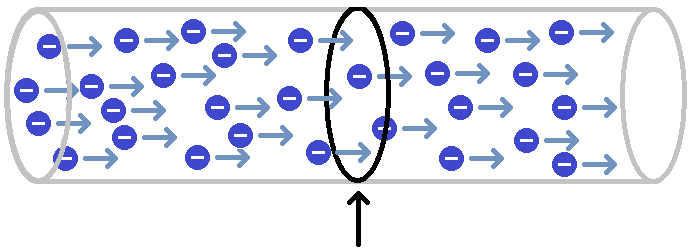
\includegraphics[width=10cm]{figures/electronFlow.png}
\caption{Electrons on-the-move! This is just an artistic rendition of what flowing charge in a wire looks like.}
\label{movingChargeThroughHoop}
\end{figure}
This brings us to the \textbf{Ampere (A)}. The ampere (or amp) is a unit that helps us describe how fast charge is moving, and its definition is 1A = 1C/1s. The diagram in Figure \ref{movingChargeThroughHoop}, which depicts electrons flowing through a section of wire, may help you visualize this. The electrons in this diagram are all flowing in the same direction, and the value of their resulting current is given by the total amount of charge that flows past a given point (denoted by the black arrow) in one second. Practically speaking, a 1A current is relatively large, especially in the context of consumer electronics like a smartphone or your computer. For historical reasons\footnote{Ben Franklin was involved, y'all.} conventional current flow is in the opposite direction of electron flow. This mostly has to do with the fact that the charge of an electron is negative, which wasn't realized until the standard for current flow was set. Don't fret, though---after this section, we will only talk about conventional current flow in this class. 
\par
Electrons must be moving to establish current, which means those electrons need kinetic energy. That kinetic energy is imparted to electrons by \textit{voltage} sources, which provide an electric potential energy difference in units of \textbf{Volts (V)}, where 1V=1J/1C. A voltage difference is to electrons like a hill is to a ball. If you put a ball up on a hill, it will start rolling down, gaining kinetic energy as its height decreases. Similarly, if you put an electron at a low voltage, it will drift toward a higher voltage. This low-to-high movement is caused by the fact that the electron's charge is negative. Don't get too hung up on the analogy; just remember that conventional current flows from the positive voltage to the negative voltage of a power supply. 
\par
In a circuit, any point at which multiple (two or more) elements are connected is referred to as a \textbf{node}, and every node has a single voltage. When we refer to voltage, we either do so in terms of voltage \textit{differences} between nodes, or we talk about a voltage in a circuit with respect to a reference node called the \textbf{ground} node.
\par
You have probably already seen power in at least one other course, but as I mentioned in the last chapter, it's a big reason why we have circuits at all. Power is the amount of energy that is supplied by a power source or \textit{dissipated} (i.e., used up) by a circuit element over time. Power is measured in \textbf{Watts (W)}, where 1W = 1J/1s. Using your dimensional analysis skills, you can confirm that power (P) is related to current (i) and voltage (V) by the following expression, known as \textit{Watt's Law}:
$$
P = i\times V
$$
\par
In words, this states that the power (in Watts) dissipated or supplied by an element is given by the current flowing through that element multiplied by the voltage across that element. 

\begin{figure}[h!]
\centering
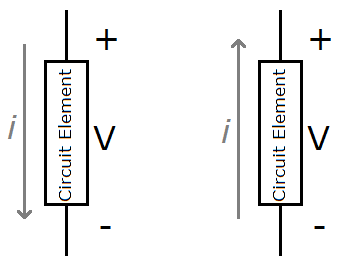
\includegraphics[width=10cm]{figures/powerSuppliedDissipated.png}
\caption{The element on the left side of this figure is dissipating power, because the current is flowing through the element from its higher voltage side to its lower voltage side. Conversely, the element on the right side of this figure is supplying power in the circuit, because the current is flowing through the element from its lower voltage side to its higher voltage side.}
\label{powerSuppliedDissipated}
\end{figure}

If the current is going in the direction of the voltage drop across the element---that is, into the terminal with greater voltage and out of the terminal with smaller voltage---then the element is dissipating that power. If the current flows in the opposite direction through the element, then that element is supplying power. Figure \ref{powerSuppliedDissipated} illustrates this convention. In either case, $V$ represents the voltage \textit{across} the source or element, and $i$ represents the current flowing \textit{through} the source or element.
\par
To facilitate the introduction of the last unit of this chapter, we need to look at a circuit. Figure \ref{resistorBatteryCircuit} shows the simplest circuit I could come up with to introduce \textit{resistance}.
\begin{figure}[h!]
\centering
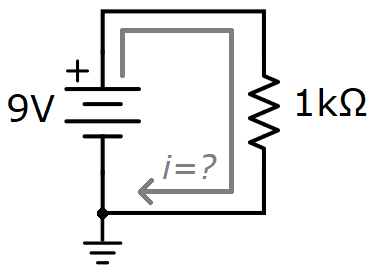
\includegraphics{figures/batteryResistorCircuit.png}
\caption{A simple circuit with a battery and a single resistor. The current in this circuit flows in the direction of the arrow.}
\label{resistorBatteryCircuit}
\end{figure}
Before we proceed, let's dissect this schematic a bit. In this circuit, there is a battery---represented by four horizontal lines and a plus sign---and a \textit{resistor}---the zig-zagged symbol on the right-hand side of the schematic. All of the straight lines that connect the elements in the circuit can be thought of as wire; these are the \textit{nodes} of the circuit. There is also a symbol at the bottom left of the circuit with three horizontal black lines that cross a vertical line connected to the bottom left node of the circuit. This symbol marks the ``ground'' node. It is common practice to include a circuit ground in schematics; ground is treated as the 0V reference for the circuit, which makes calculations and debugging easier. 
\par
The battery is labeled ``9V'', meaning there is a 9 volt \textit{difference} between its positive and negative (top and bottom) terminals. This also means there is a 9V difference between the nodes connected to its positive and negative terminals. 
\par
The gray arrow denotes the direction of current flow in this circuit---out of the positive terminal of the battery, through the resistor, and into the negative terminal of the battery. The value of the current is the same at all points along this loop.
\par
%Ohm's law
The resistor is labeled ``1k$\Omega$'', which is its resistance in \textbf{Ohms ($\Omega$)}. The \textbf{Ohm} is the unit of resistance (or impedance), and it relates the current flowing through an element to the voltage difference across that element. Initially, this unit was defined empirically upon the observation that voltage and current are approximately linearly proportional in most materials. Dimensionally, the Ohm is defined according to the following relationship:
$$
1\Omega = \frac{1V}{1A}
$$
\par
In order to determine the value of the current flowing in this circuit, we will need to use \textbf{Ohm's Law}:
$$
V=i \times R
$$
In words, this law states that the voltage difference across (or the voltage drop over) the resistor is equal to the value of the current flowing through the resistor (represented as $i$) multiplied by the resistance of the resistor ($R$). The voltage across the resistor is defined by the battery as 9V. Since we know the value of the resistance is 1000$\Omega$, we can rearrange Ohm's law to find the value of the current flowing through the resistor:
$$
i = \frac{9\textrm{V}}{1000\Omega} = 0.009 \textrm{A}
$$
Figure \ref{resistorBatteryCurrentCircuit} shows the fully-annotated schematic for this circuit.
\begin{figure}[h!]
\centering
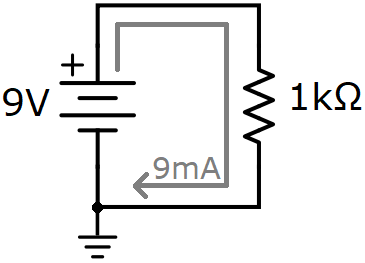
\includegraphics{figures/batteryResistorCurrentCircuit.png}
\caption{The circuit of Figure \ref{resistorBatteryCircuit}, with current labelled.}
\label{resistorBatteryCurrentCircuit}
\end{figure}
\par
To save time later, I will use the prefixes M ($10^6$), k ($10^3$), m ($10^{-3}$), $\mu$ ($10^{-6}$), n ($10^{-9}$), and p ($10^{-12}$)to represent orders of magnitude for the quantities we calculate. Current is usually on the order of $10^{-3}$A, or mA, and resistors are often on the order of $10^{3}\Omega$, or k$\Omega$. The nice thing about these unit prefixes is that they cancel each other out when multiplied: 1mA$\times$1k$\Omega$ = 1A$\times$1$\Omega\times\cancel{10^3\times10^{-3}}$ = 1V. They also often convert to one another in calculations through the property that $\frac{1}{m} \rightarrow k$ and $\frac{1}{k} \rightarrow m$. Using these prefixes, we cite the current in the circuit of Figure \ref{resistorBatteryCurrentCircuit} as 9mA. The other prefixes will come up later, too, but I will try to remind you of their meaning when they do.
\par
We've now seen all the fundamental units of circuits, but let's use Watt's law to fully characterize the behavior of the circuit in Figures \ref{resistorBatteryCircuit} and \ref{resistorBatteryCurrentCircuit}. Having found the value of the current in this circuit, we have almost completely defined its behavior. However, remember that all circuits either power devices or condition signals, and even though this circuit is mostly instructive in purpose, let's assume that the whole point of this circuit is to provide power to the resistor. If that's the case, we need to determine how much power the resistor is receiving. To do so, we will rely on Watt's Law. Looking again at our circuit in Figure \ref{resistorBatteryCurrentCircuit}, if the voltage across the resistor is 9V and the current through the resistor is 9mA, then the power dissipated by the resistor is $9\textrm{mA}\cdot9\textrm{V} = 81\textrm{mW}$. Likewise, since there are 9V across the battery terminals and the current flowing through the battery is 9mA, the battery is \textit{supplying} 81mW. It is always good to verify that the power supplied by the sources in a circuit is equal to the power dissipated by the elements of a circuit; this is a good way to double-check your calculations. Energy is always conserved, after all...even in circuits!
\par
Before moving on, let's use Ohm's law to generate two additional forms of Watt's Law. If we combine Ohm's law with Watt's law, we can derive the following alternate form for Watt's law:
$$
P = i\times V = i\times(i\times R) = i^2\times R
$$
Additionally, if we rearrange Ohm's law as i = $\frac{V}{R}$, then we can use this definition of current in Watt's law in the following way:
$$
P = i\times V = \frac{V}{R}\times V = \frac{V^2}{R}
$$

In analyzing circuits, you will sometimes find one of these forms of Watt's Law to be more useful than the others. You should be able to quickly recall all of these forms or at least derive them.
\subsection{More Schematic Symbols for Power Supplies}
The example circuit in Figure \ref{resistorBatteryCurrentCircuit} includes a battery, which is one type of DC power supply. There are two other symbols for DC supplies you should know about so that when they come up in future chapters you won't be lost. 
\begin{figure}[h!]
\centering
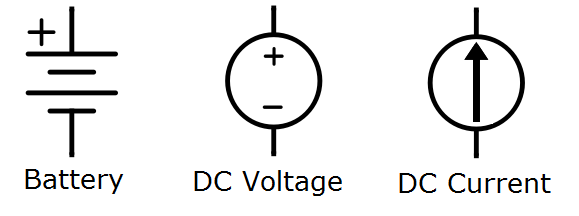
\includegraphics{figures/DCpowerSupplies.png}
\caption{Common DC power supply symbols.}
\label{DCpowerSupplies}
\end{figure}
\par
Figure \ref{DCpowerSupplies} shows all the types of DC power supplies you can expect to see in this course. (There are AC power supplies, too, but those will be introduced in Chapter \ref{chap:ACcircuits}.) The symbol on the far left of this figure represents a battery, which we have already seen. Batteries provide a constant voltage difference between their two terminals. The circular symbol in the middle of Figure \ref{DCpowerSupplies} with terminals marked ``+'' and ``-'' represents a DC voltage supply more generally; it could represent any regulated DC voltage supply or a battery. The circular symbol on the far right of the figure with an arrow running from one of its terminals to the other represents a DC current source. For powering electronics, voltage sources are superior to and far more prevalent than DC current sources. As a result, there are not many examples of DC current sources in your everyday life, with one notable exception---your phone charger. Like most battery chargers, a phone charger provides a steady current in reverse through the battery in order to put charge carriers back into the negative terminal of the battery. We will use current sources in calculations at times in this course, but they are more useful and practical in circuit analysis than in everyday use.

\section{(Additional) Fundamental Laws}
In the process of introducing the basic units of circuits in the previous section, I also introduced two of the most import laws of circuits---Ohm's and Watt's Laws. In this section, I will introduce the two remaining fundamental laws of circuits---Kirchhoff's Current Law and Kirchhoff's Voltage Law---by deriving them while we investigate the properties of two more circuits.
\begin{figure}[h!]
\centering
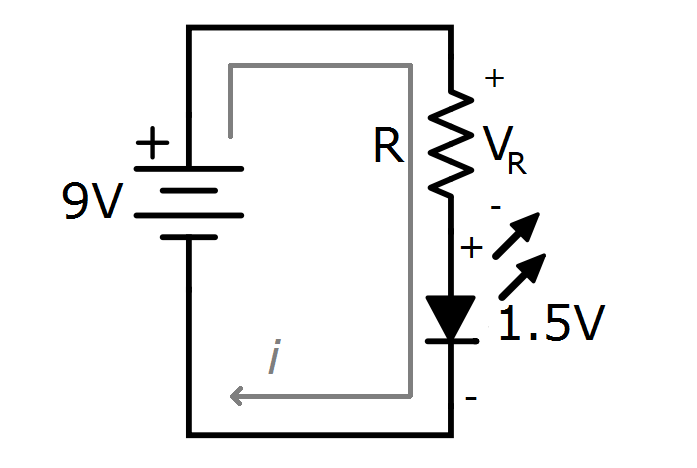
\includegraphics[width=10cm]{figures/LEDCircuit.png}
\caption{A circuit that lights up an LED.}
\label{simpleLED}
\end{figure}

The circuit of Figure \ref{simpleLED} is designed to light up (provide power to) a light-emitting diode (LED) without destroying it. There are only three elements in this circuit: a battery, a resistor, and an LED (whose symbol looks like a big arrow pointing directly at a line, with little floating arrows above and to the right of it). Let's assume that the LED can handle at most 30mW, and that we need to find a value for resistor ``R'' that will ensure this power limit is obeyed. The battery voltage is 9V, the resistor has a resistance of \textit{R}, and the LED, when operating, has a constant 1.5V across it\footnote{I'm not going to describe how LEDs physically work in this class, but when an LED is emitting light, we can assume there is some constant voltage across it. 1.5V is a realistic voltage, but different LEDs can have different voltage values depending on the color and fabrication parameters of the LED.}. The current, $i$, is shown in gray.  If I want to know how much power the LED is using, I just need to know the voltage across it and the current flowing through it. Then I can use Watt's Law to solve for the power being dissipated by the LED. For the circuit of Figure \ref{resistorBatteryCircuit}, I knew the voltage across the resistor and the resistance itself, and that information allowed me to use Ohm's law ($V=i \times R$) to find the current flowing through that circuit. In the circuit of Figure \ref{simpleLED} however, the voltage across the resistor is not given. To find it, we need to use \textbf{Kirchhoff's Voltage Law} (which I will refer to as \textbf{KVL} from now on):
$$
\textrm{Around any loop in a circuit,} \sum\textrm{\{voltage added\}} = \sum\textrm{\{voltage dropped\}}
$$
Or, in shorthand, 
$$
\sum_{loop}\Delta V^+ = \sum_{loop}\Delta V^- \textrm{  or simply }\sum_{loop}\Delta V = 0
$$
In words, this states that if I trace through a complete loop (starting and stopping at the same node) of a circuit, I will encounter voltage drops and voltage increases, and for any such loop, the amount of voltage dropped will be equal to the amount of voltage added. If I trace clockwise through the circuit of Figure \ref{simpleLED} starting at the bottom left corner, I encounter the 9V increase of the battery, then an unspecified voltage drop across the resistor, and then the 1.5V drop across the LED, which takes me back to the node where I started. The increases in voltage and the voltage drops in that loop should sum to zero. Writing this out as an equation,
$$
9\textrm{V} - V_R - 1.5\textrm{V} = 0
$$
From this equation we see that the voltage drop across the resistor, $V_R = 7.5\textrm{V}$.
\par
With the voltage across the resistor determined, we can solve for the current flowing through the resistor and the LED in terms of the resistance, $R$. Remember that the purpose of this circuit is to provide power to the LED \textit{without destroying it}, and that the LED can handle \textit{at most} 30mW. If that's the case, then according to Watt's Law, the following expression must be true:
$$
1.5V \cdot i \leq 30\textrm{mW}
$$
To enforce this requirement, we must set $R$ so that the current does not exceed 30mW/1.5V, or 20mA. Using this expression for current and the fact that $V_R=7.5\textrm{V}$ along with Ohm's law, we can set a \textit{lower-bound} (R$_{min}$) on the range of allowable values for $R$ in the following way:
$$
7.5\textrm{V} = i \times R_{min} = 20\textrm{mA} \cdot R_{min},
$$
therefore
$$
R_{min} = \frac{7.5\textrm{V}}{20\textrm{mA}} = 375\Omega
$$
\par
So, in order for the LED in Figure \ref{simpleLED} to light up and not \textit{burn} up, the resistor value must be \textit{at least} 375$\Omega$. If you followed along with this example, congratulations! You just experienced a taste of electric circuit design!
\par
%KCL
There is one last fundamental law to introduce, and to do so we will look at the circuit of Figure \ref{twoLEDs}.
\begin{figure}[h!]
\centering
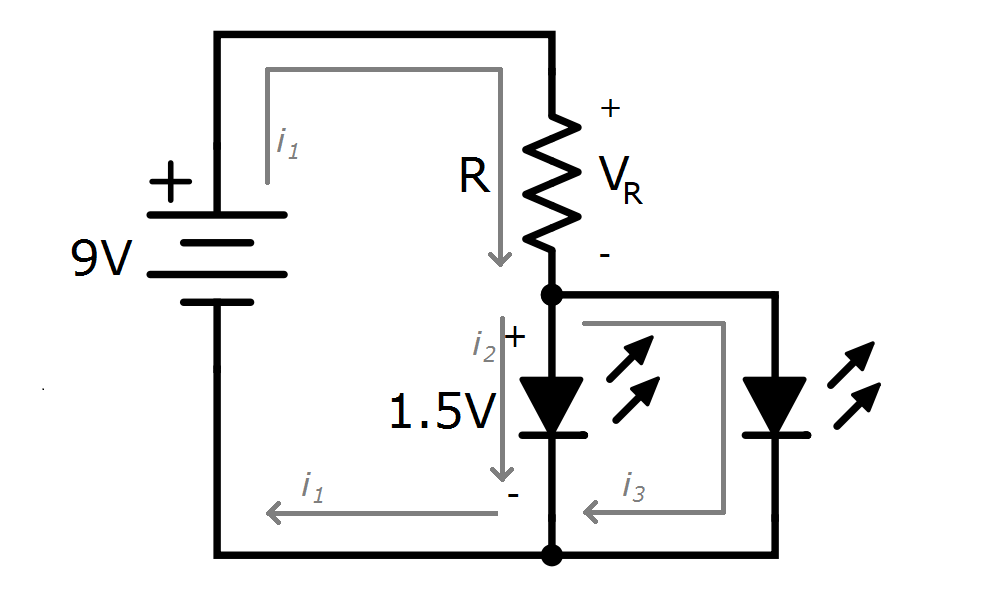
\includegraphics[width=12cm]{figures/twoLEDsCircuit.png}
\caption{A circuit that lights up two LEDs.}
\label{twoLEDs}
\end{figure}

This circuit is comprised of a battery, a resistor, and two LEDs. As before, the voltage across both of the LEDs is 1.5V, and KVL tells us that the voltage across the resistor must be 7.5V. However, this circuit has more than just one full loop. The dot connecting the resistor and the two LEDs indicates that all three wires converging there form a node. At that node, current $i_1$ enters from the resistor branch and currents $i_2$ and $i_3$ exit through the two LED branches. We can relate these three currents usign \textbf{Kirchhoff's Current Law} (which I will refer to as \textbf{KCL} from now on): 
$$
\textrm{At any node in a circuit,} \sum\textrm{\{current entering\}} = \sum\textrm{\{current leaving\}}
$$
Or, in shorthand
$$
\sum_{node}i_{in} = \sum_{node}i_{out}
$$

In words, this means that the amount of current flowing into a node must be equal the amount of current flowing out of that node. In our circuit, this means that $i_1=i_2+i_3$. Let's assume that both LEDs are identical, and therefore the current flowing through each LED is the same. In that case, $i_2=i_3$. Let's also assume that we need to enforce the same constraints on the power delivered to each LED as before---$P_{LED}\leq30\textrm{mW}$. Therefore, the current flowing through each LED must be constrained to be 20mA or less (we'll define $i_{2,max}=20\textrm{mA}$ and $i_{3,max}=20\textrm{mA}$). If we assume that each of these currents is at its maximum value, then $i_2=i_3=20\textrm{mA}$ and according to KCL, the maximum value for the current flowing through the resistor in this circuit $i_{1,max}=i_{2,max}+i_{3,max}=40\textrm{mA}$. As was the case in our analysis of the circuit in Figure \ref{simpleLED}, this maximum current value places a constraint on the possible resistance values of our resistor; given the fact that the voltage across the resistor is set at 7.5V, according to Ohm's Law, $R_{min}=7.5V/i_{1,max}=187.5\Omega$. This is half of the minimum resistance value we found for the circuit of Figure \ref{simpleLED}; why do you think that is?
\section{Recap: The Fundamentals}
In the previous section, I introduced several fundamental concepts without dwelling too much on definitions. I want to ennumerate and concisely define each of these concepts here again:
\begin{description}
\item[Charge] is measured in \textit{Coulombs} (C) and is the foundational measure of electronics. An electron has a charge of -1.602$\times10^{-19}$C, which means that a single negative coulomb is made up of LOTS of electrons.

\item[Current] is measured in \textit{Amperes} (A) (or just \textit{Amps}) and is defined as the flow of charge through an element or elements. Dimensionally, 1A=1C/1s. Current that flows through a single branch has a constant value at all points along that branch.

\item[Nodes] are points in a circuit at which multiple (two or more) elements are connected. Each node has a constant voltage.
\item[Ground] is the node in a circuit with respect to which all other node voltages are referenced; if a specific voltage value is cited at a point in a circuit, that is usually relative to ground.

\item[Voltage] is measured in \textit{Volts} and is defined as energy per unit charge. Dimensionally, 1V=1J/1C. We often refer to voltage \textit{across} an element; by this, we mean the \textit{difference} between the voltages at the two ends of that element. We also sometimes refer to voltage at a node with respect to the voltage at another node, usually the \textit{ground} node.

\item[Power] is measured in \textit{Watts}, and is defined as energy supplied or dissipated over time. Dimensionally, 1W=1V$\cdot$1A.\footnote{1W=1J/1s of course, but the definition above is generally more useful for this course. The standard definition can be derived from 1W=1V$\cdot$1A without too much effort.} Power in circuits is typically supplied by voltage or current sources and dissipated by resistors.

\item[Watt's Law] is the name for the law that relates power supplied or dissipated by a circuit element to the current flowing through that element and the voltage across that element. Through the use of Ohm's Law, several forms of Watt's Law can be derived: 
$$
P = i \times V = i^2 \times R = \frac{V^2}{R}
$$

\item[Resistance] is measured in \textit{Ohms}, and it relates the voltage across a resistor to the current flowing through that resistor. Dimensionally, $1\Omega$=1V/1A. Resistance is the real (as opposed to imaginary) part of a broader relationship between current and voltage known as \textit{impedance}, which we will introduce later in the course.

\item[Ohm's Law] is related to resistance, and it states that the value of the voltage across a resistive element is equal to the value of the current flowing through that element multiplied by the resistance of that element:
$$V=i \times R$$

\item[Kirchhoff's Voltage Law (KVL)] states that around any loop in a circuit, the voltage added is equal to the voltage dropped:
$$\sum_{loop}{\Delta V^+} = \sum_{loop}{\Delta V^-}$$
This law is an expression of the concept of conservation of energy; all the energy delivered to a circuit must be dissipated by that circuit.
\item[Kirchhoff's Current Law(KCL)] states that at any node in a circuit, the current flowing in is equal to the current flowing out:
$$\sum_{node}{i_{in}} = \sum_{node}{i_{out}}$$
This law is an expression of the concept of conservation of mass; however many electrons flow into a node must also flow out of that node.
\end{description}
\par
These concepts may seem overwhelming all at once, but everything we do now will rely on these. If you read this whole chapter, you have now seen \textit{every} fundamental concept pertaining to electric circuits.
\chapter{Helpful Rules and Tricks for Resistor Circuits}
\label{chap:resistorRulesAndTricks}
In this chapter, I'll finalize some terminology we'll use a lot in this course, and then we're going to use the laws we saw in Chapter \ref{chap:fundamentals} to derive some rules that will simplify the process of analyzing circuit behavior. The rules and tricks derived in this chapter can help you see past the density of elements in some circuits to discern their underlying functionality. Furthermore, even though we are working in the context of resistors exclusively, the applicability of this material extends to all passive elements (resistors, capacitors, and inductors), which we will see later in the course.
 
\section{Circuit Terminology}
Before we proceed, I need to introduce some circuit concepts. I will use these terms from now on, so it's important that we all know what they mean.
\begin{figure}[h!]
\centering
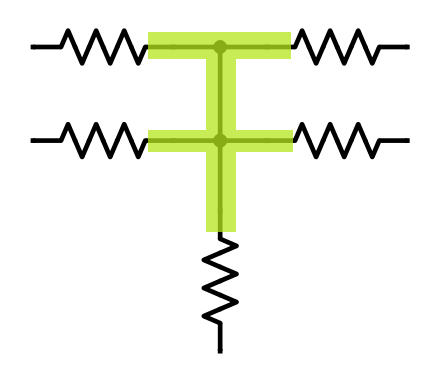
\includegraphics[width=13cm]{figures/nodeCloseUp.png}
\caption{The highlighted common connection that these resistors share is an example of a \textit{node}.}
\label{nodeCloseUp}
\end{figure}
\par
I introduced \textbf{nodes} in Chapter \ref{chap:fundamentals}, but their definition bears repeating and expanding; a \textbf{node} is a place in a circuit where two or more elements are connected. An example of a node is highlighted in Figure \ref{nodeCloseUp}. At any node, there is just one voltage value. All the nodes of the circuit in Figure \ref{nodesHighlighted} have been highlighted. You can see that nodes can be simple or elaborate in shape, but being able to determine how many nodes are in a circuit is an important skill.
\begin{figure}[h!]
\centering
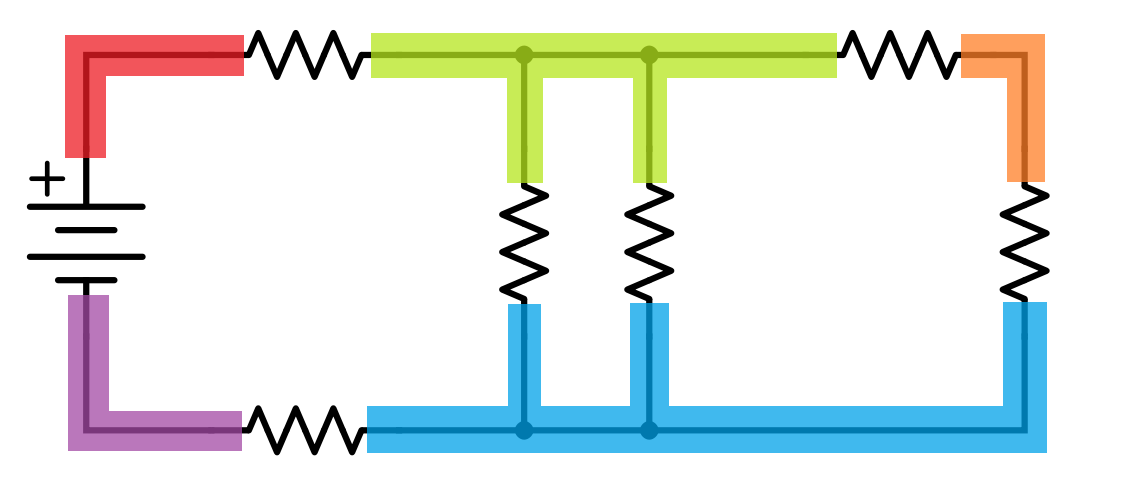
\includegraphics[width=13cm]{figures/nodesHighlighted.png}
\caption{The nodes in this circuit are each highlighted in a different color.}
\label{nodesHighlighted}
\end{figure}

\par
A \textbf{branch} is simply a connection that allows current to flow between nodes. Branches are comprised of circuit elements like resistors and power supplies. The branches of the circuit in Figure \ref{branchesHighlighted} are highlighted. When I use the term \textbf{branch}, I mean a single path for current to flow through, and one branch could be comprised of several elements depending on the context. For example, in Figure~\ref{branchesHighlighted}, the leftmost three elements of the circuit together comprise a branch. Similarly, the rightmost two resistors in Figure~\ref{branchesHighlighted} comprise another branch.
\begin{figure}[h!]
\centering
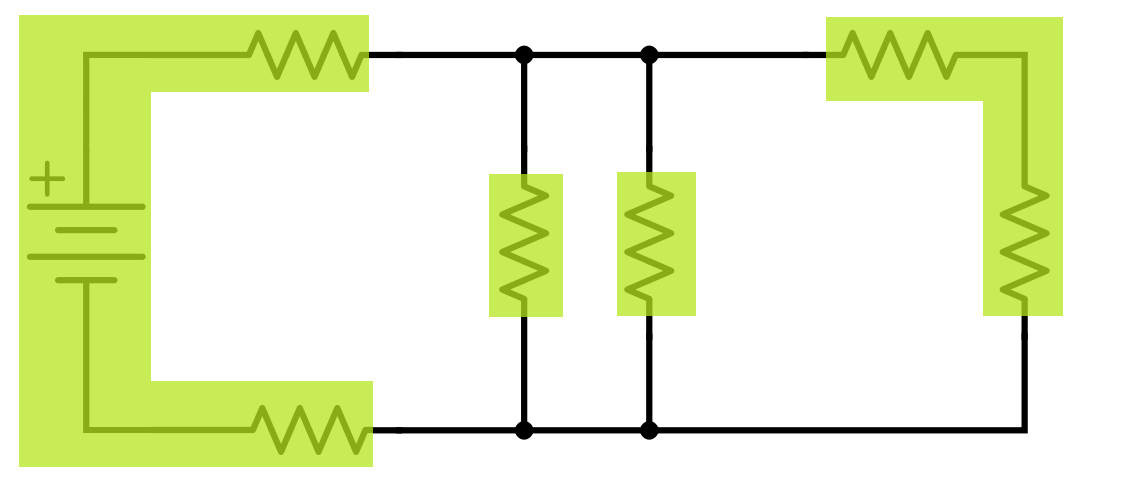
\includegraphics[width=13cm]{figures/branchesHighlighted.png}
\caption{The branches in this circuit are each highlighted.}
\label{branchesHighlighted}
\end{figure}

\par
If I describe several elements as being \textbf{in series}, that means that there is a single path for current to flow through them; in other words, they are connected head-to-tail, with only two elements sharing each node in the series connection. Two resistors in series have been highlighted in the circuit of Figure \ref{seriesHighlighted}. There is only one path for current to flow through those two elements, and there are no other branches connected to their shared node.
\begin{figure}[h!]
\centering
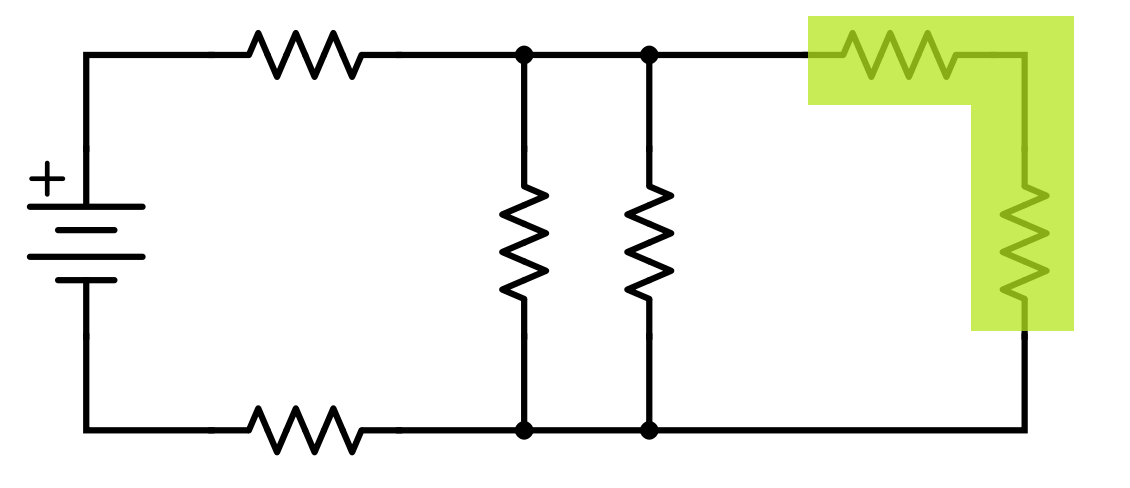
\includegraphics[width=13cm]{figures/seriesHighlighted.png}
\caption{The two highlighted resistors in this circuit are in series.}
\label{seriesHighlighted}
\end{figure}
\par
\textbf{Parallel} elements share both of their nodes with each other. Two parallel resistors are highlighted in the circuit of Figure \ref{parallelHighlighted}. We know these resistors are in parallel because they share both of their nodes.
\begin{figure}[h!]
\centering
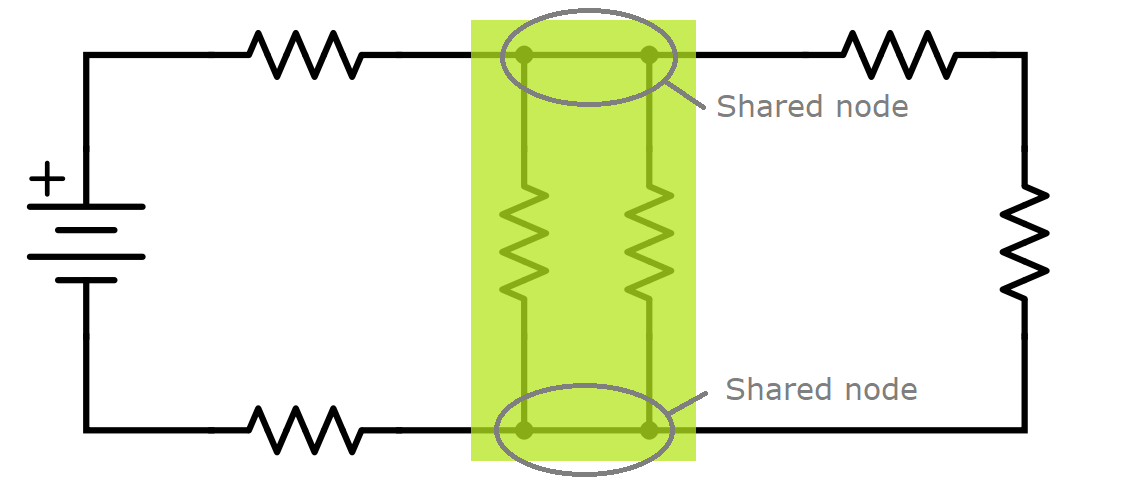
\includegraphics[width=13cm]{figures/parallelHighlighted.png}
\caption{The two highlighted resistors in this circuit are in parallel. We can tell this, because their head and tail nodes are shared.}
\label{parallelHighlighted}
\end{figure}
\par
Now that we have defined these terms, it's time to learn some rules and tricks for simplifying circuit analysis.

\section{Using Ohm's Law to Define Resistance}
Ohm's Law states that the voltage across a resistor is equal to to the value of the current flowing through that resistor multiplied by its resistance ($V = i \cdot R$). From this law, we could also define resistance of any general circuit element or collection of elements in a circuit as the ratio of the voltage across it divided by the current flowing through it, as shown in Figure \ref{genericElementResistance}. 
\begin{figure}[h!]
\centering
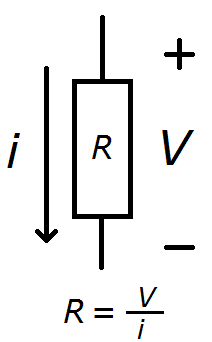
\includegraphics[width=3cm]{figures/singleElementRes.png}
\caption{The resistance of a circuit element or a collection of elements is defined as $R = V/i$ according to Ohm's law.}
\label{genericElementResistance}
\end{figure}

The circuits we have seen so far have had just a single resistor, but most real circuits have dozens or more. Any grouping of resistors can be simplified by finding an equivalent resistance for the entire collection.


\section{Equivalent Resistance of Series Resistors}
\label{sec:seriesEquivalent}
Let's consider a section of a circuit comprised of two resistors connected in series like that shown in Figure \ref{twoSeriesToEquivalent}. If we want to simplify a series of resistances like this into a single equivalent resistance, all we need to do is determine the value of the current flowing  through the resistors and then calculate the ratio of the voltage across them ($V_s$ in this case) to that current. 
\begin{figure}[h!]
\centering
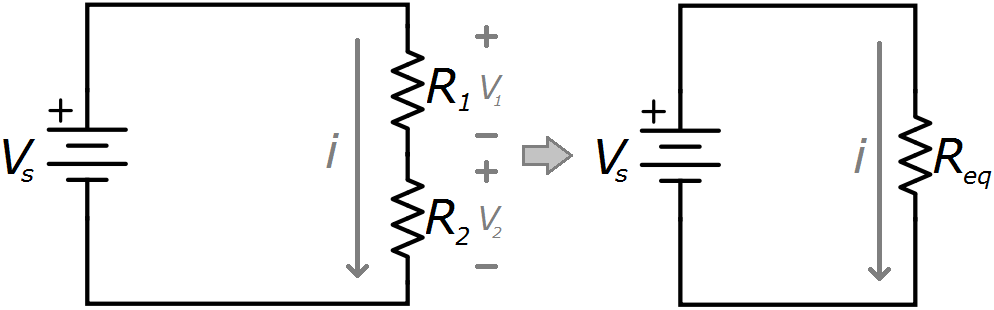
\includegraphics[width=13cm]{figures/twoResSeries.png}
\caption{The current flowing through two resistors in series and the voltage across both define their equivalent resistance.}
\label{twoSeriesToEquivalent}
\end{figure}
We can relate the voltage drops across each resistor (which I have labelled $V_1$ and $V_2$) and the source voltage using Kirchhoff's Voltage Law: $V_s = V_1 + V_2$. We can further define $V_1$ and $V_2$ in terms of the current flowing through the branch, $i$ and the respective resistances as $V_1 = i \cdot R_1$ and $V_2 = i \cdot R_2$. We also know that the current flowing through each resistor is the same, and we can define it as $i = \frac{V_s}{R_{eq}}$. Putting these expressions together and manipulating them algebraically yields the following:
$$
i = \frac{V_1 + V_2}{R_{eq}} = \frac{i \cdot R_1 + i \cdot R_2}{R_{eq}} = \frac{i(R_1+R_2)}{R_{eq}}
$$
$$
\textrm{     therefore     }R_{eq} = \frac{\bcancel{i}(R_1+R_2)}{\bcancel{i} \cdot R_{eq}} = R_1 + R_2
$$

Therefore, the equivalent resistance for the series of resistors $R_1$ and $R_2$ is given by their sum. This is the simplest specific case of the general rule for combining resistors in series:
$$
\textnormal{For any series of resistors    } R_1, R_2,\dots, R_n, \textnormal{   }R_{eq} = \sum_{i=1}^n{R_i}
$$
%parallel
\section{Equivalent Resistance of Parallel Resistors}
\label{sec:parallelResistors}
We can also calculate the equivalent resistance of parallel resistors. A pair of parallel resistors is shown in Figure \ref{twoParallelToEquivalent}. 
\begin{figure}[h!]
\centering
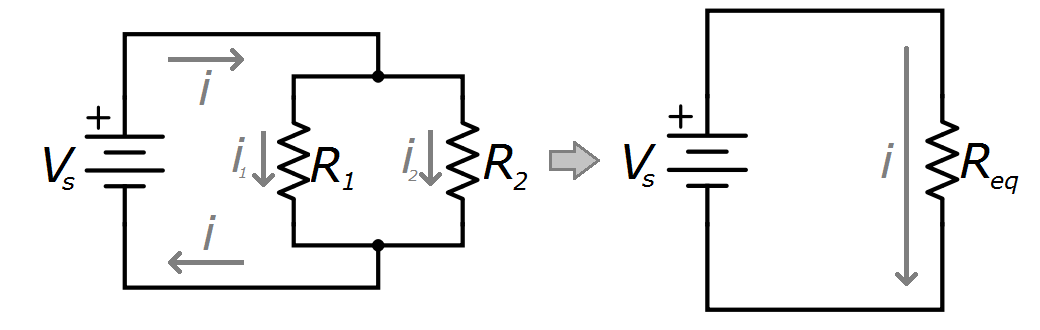
\includegraphics[width=13cm]{figures/twoResParallel.png}
\caption{Current flowing into two resistors in \textit{parallel} (i.e., sharing both head and tail nodes) and the voltage across them define their equivalent resistance.}
\label{twoParallelToEquivalent}
\end{figure}
This time, to determine the expression for $R_{eq}$, we will first use Kirchhoff's Current Law to relate $i$, the current coming from the source, to the labelled currents $i_1$ and $i_2$: 
$$i = i_1 + i_2$$
We know this is true, because current entering a node must be equal to the current leaving a node, and at the node above resistors $R_1$ and $R_2$, $i$ enters from the top, and $i_1$ and $i_2$ flow down through $R_1$ and $R_2$.
\par
Next, because these resistors share their head and tail nodes, we know that the voltage across $R_1$ is equal to the voltage across $R_2$. Furthermore, since $V_s$ is connected across both resistors, we know that the voltage across each resistor is just $V_s$. We can use this fact along with Ohm's Law to determine expressions for $i_1$ and $i_2$:
$$
V_s = i_1\cdot R_1\textnormal{, so   }i_1 = \frac{V_s}{R_1}
$$
and similarly
$$
i_2 = \frac{V_s}{R_2}
$$
Combining these expressions for current with  the expressions above and the fact that $R_{eq} = \frac{V_s}{i}$ yields the following:
$$
R_{eq} = \frac{V_s}{i_1 + i_2} = \frac{V_s}{\frac{V_s}{R_1} + \frac{V_s}{R_2}} = \frac{\bcancel{V_s}}{\bcancel{V_s}\cdot(\frac{1}{R_1} + \frac{1}{R_2})} = \frac{1}{\frac{1}{R_1} + \frac{1}{R_2}}
$$
In general, for parallel resistors $ R_1, R_2,\dots, R_n,$ 
$$
R_{eq} = \frac{1}{\displaystyle\sum_{i=1}^n{\left(\frac{1}{R_i}\right)}}
$$
\par
In the special case of just two resistors in parallel---$R_1$ and $R_2$ in our example---we can always use the equivalent resistance
$$
R_{eq} = \frac{R_1R_2}{R_1+R_2}
$$
which is a convenient expression to remember.

%Voltage divider rule
\section{Voltage Dividers}
\label{sec:voltageDividers}
\begin{figure}[h!]
\centering
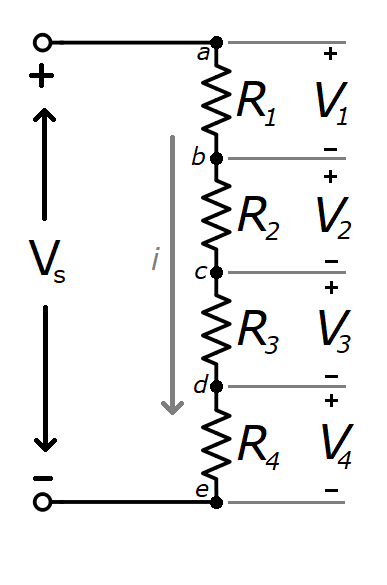
\includegraphics[width=5cm]{figures/voltageDivider.png}
\caption{These resistors in series form a voltage divider; they divide the voltage $V_s$ into four smaller voltages.}
\label{voltageDivider}
\end{figure}
Many circuits use resistors in series to reduce a voltage by some amount or to divide a voltage into smaller voltages. Because of this, a series connection of resistors is referred to as a \textbf{voltage divider}. An example voltage divider is shown in Figure \ref{voltageDivider}, and it divides the voltage $V_s$ into the four voltages $V_1$, $V_2$, $V_3$, and $V_4$. The values of these four voltages can be determined in terms of $V_s$ and the resistances $R_1$, $R_2$, $R_3$, and $R_4$ using the \textbf{Voltage Divider Rule}, which we will derive now using Figure \ref{voltageDivider}.
\par
First, let's assume there is an unknown current, $i$, flowing through the resistors in Figure \ref{voltageDivider} from top to bottom. In terms of that current and the resistances, Ohm's law tells us that the voltages across the four resistors are defined as 
$$
V_1 = i \cdot R_1
$$
$$
V_2 = i \cdot R_2
$$
$$
V_3 = i \cdot R_3
$$
$$
V_4 = i \cdot R_4
$$
We want to get rid of the current $i$ in our definitions for these voltages, because $i$ was not initially given and we should always find expressions in terms of variables that were defined in the initial circuit. In this case, we want our definitions for the voltages across each of the resistors to be given in terms of just the resistances in the circuit.
\par
In section \ref{sec:seriesEquivalent}, we learned that the equivalent resistance of all of the series of resistors in this voltage divider can be expressed as $R_{eq}=R_1 + R_2 + R_3 + R_4$. Then, Ohm's law tells us that $V_s = i \cdot R_{eq}$, and we can therefore define $i$ in terms of $V_s$ and $R_{eq}$ in the follwing way: 
$$
i=\frac{V_s}{R_{eq}}
$$
Folding this representation of $i$ into the expressions for voltages across the resistors yields
$$
V_1 = V_s \cdot \left(\frac{R_1}{R_{eq}}\right)
$$
$$
V_2 = V_s \cdot \left(\frac{R_2}{R_{eq}}\right) 
$$
$$
V_3 = V_s \cdot \left(\frac{R_3}{R_{eq}}\right)
$$
$$
V_4 = V_s \cdot \left(\frac{R_4}{R_{eq}}\right)
$$

I hope from these expressions you detect the pattern. Each of these are manifestations of the \textbf{Voltage Divider Rule}, which can be used to determine the voltage across any resistor in a voltage divider (which is really just a series of resistors):
$$
\mathlarger{\mathlarger{\mathlarger{V_n = V_s}}} \cdot \left(\frac{R_n}{\displaystyle\sum_{i=1}^m{R_i}}\right)
$$
This rule follows from the fundamental concepts of Chapter \ref{chap:fundamentals} and it is extremely useful. Once you get comfortable with the voltage divider rule, you will start to see voltage dividers in most circuits you encounter. When we start looking at time-varying (AC) voltages, capacitors, and inductors, we will find even more uses for the voltage divider rule in defining circuit behavior.

%Current divider rule
\section{Current Dividers}
\label{sec:currentDividers}
Parallel configurations of resistors are sometimes referred to as current dividers. I don't find these as useful as voltage dividers, but they do crop up in many circuits. Like in the last section, we will focus on a specific circuit---that of Figure \ref{currentDivider}---to derive a general rule for analyzing these circuit configurations.
\begin{figure}[h!]
\centering
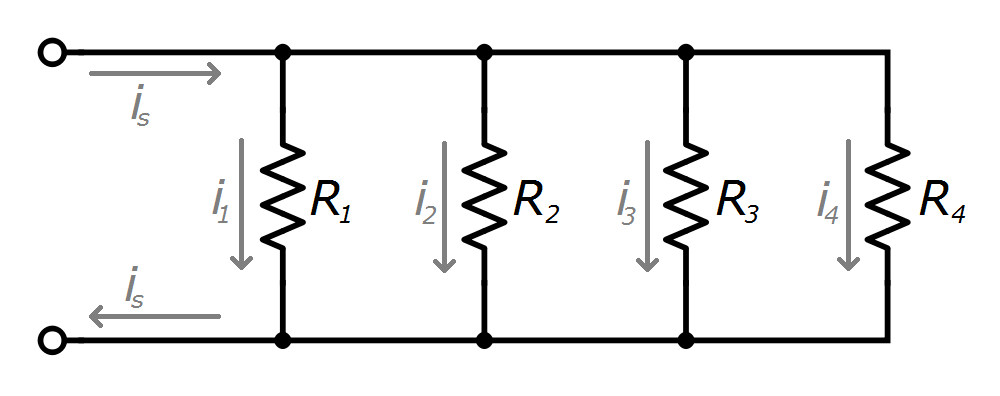
\includegraphics[width=10cm]{figures/currentDivider.png}
\caption{These resistors in parallel form a current divider; they divide the current $i_s$ into four smaller currents.}
\label{currentDivider}
\end{figure}
\par
Let's start off by assuming there is an unknown voltage $V$ across all four resistors in Figure \ref{currentDivider}. We can use that voltage and Ohm's law to relate all the resistances and the currents flowing through them:
$$
V = i_1 \cdot R_1 = i_2 \cdot R_2 = i_3 \cdot R_3 = i_4 \cdot R_4
$$
From Section \ref{sec:parallelResistors}, we know that the equivalent resistance of $R_1$, $R_2$, $R_3$, and $R_4$ is defined as
$$
R_{eq} = \frac{1}{\frac{1}{R_1} + \frac{1}{R_2} + \frac{1}{R_3} + \frac{1}{R_4}}
$$
Furthermore, Ohm's law tells us that  $V=i_s \ cdot R_{eq}$. Combining this expression for V with the individual resistor expressions above yields
$$
i_s \cdot R_{eq} =  i_1 \cdot R_1 = i_2 \cdot R_2 = i_3 \cdot R_3 = i_4 \cdot R_4
$$
Rearranging these expressions yields the following definitions for the individual currents flowing through the resistors:
$$
i_1 = i_s \cdot \left(\frac{R_{eq}}{R_1}\right)
$$
$$
i_2 = i_s \cdot \left(\frac{R_{eq}}{R_2}\right)
$$
$$
i_3 = i_s \cdot \left(\frac{R_{eq}}{R_3}\right)
$$
$$
i_4 = i_s \cdot \left(\frac{R_{eq}}{R_4}\right)
$$
These expressions are specific examples of the \textbf{Current Divider Rule}, which states that
$$
\mathlarger{\mathlarger{\mathlarger{i_n = i_s}}} \cdot \left(\frac{\left(\frac{1}{\sum_{i=1}^n{\left(\frac{1}{R_i}\right)}}\right)}{R_n}\right)
$$
Using this rule allows us to determine how much current flows through individual branches in a parallel circuit without having to find the voltage across those branches.
\section{Recap: Combining Resistors in Series and Parallel, and Rules to Simplify Circuit Analysis}
In this chapter, we built on the fundamental concepts of Chapter \ref{chap:fundamentals} to derive some rules for combining resistors and for determining values for voltages or currents in specific resistor configurations. The important concepts and equations from this chapter are concisely listed below.
\begin{description}
\item[Nodes] are points in a circuit where elements are connected. Each node has a constant voltage associated with it.
\item[Branches] are the connections between nodes; these can be comprised of single circuit elements, or multiple elements in series.
\item[Series] elements are those that are connected head-to-tail and that create a single path through which current can flow.
\item[Parallel] elements share both of their nodes, and the voltage across each of the parallel elements is the same.
\item[Resistors in Series] can be reduced to a single, equivalent resistance. The resistance is the sum of the resistances in series: 
$$
\textnormal{For $m$ resistors in series,    }R_{eq} = \displaystyle\sum_{i=1}^{m}R_i
$$
\item[Resistors in Parallel] can also be reduced to a single, equivalent resistance. This resistance is defined as follows:
$$
\textnormal{For $m$ resistors in parallel,    }R_{eq} = \frac{1}{\displaystyle\sum_{i=1}^{m}\left(\frac{1}{R_i}\right)}
$$
\item[The Voltage Divider Rule] can be used to determine the voltage across a single resistor in a series of resistors without requiring the calculation of currents:$$\mathlarger{\mathlarger{\mathlarger{V_n = V_s}}} \cdot \left(\frac{R_n}{\sum_{i=1}^m{R_i}}\right)$$

\item[The Current Divider Rule] can be used to determine the current flowing through a single resistor among several resistors in parallel without requiring the calculation of the voltage across all the parallel resistors:
$$\mathlarger{\mathlarger{\mathlarger{i_n = i_s}}} \cdot \left(\frac{\left(\frac{1}{\sum_{i=1}^n{\left(\frac{1}{R_i}\right)}}\right)}{R_n}\right)$$
\end{description}

\input{ch3_5__nodeVoltageandMeshCurrentAnalysis.tex}
\chapter{Power Delivery and Equivalent Circuits}
\label{chap:powerSuppliesDelivery}
Remember that one of the main purposes of electric circuits is to deliver power to devices. Often, we call these devices \textbf{loads}, because they load down a circuit by drawing power from that circuit. In order to maximize the amount of power that is delivered to a load from a particular circuit, we need to use some math to determine what the resistance of that load should be. Or, if the resistance (or impedance) of the device we are interested in powering is known, we need to design its driving circuitry according to that known load resistance (or impedance). Either way, the material covered in this chapter will facilitate those design decisions.
\par
\section{Driving Circuit for a Load}
In this chapter, I will refer to \textbf{driving circuits} for loads. By this, I mean everything in a circuit \textit{besides} the load in question. Consider Figure \ref{maxPowerLoadMatching}. This figure shows a simple driving circuit (encircled in the figure by a gray box) that powers a load. The internal voltage source for the driving circuit is denoted as $V_s$, the internal resistance for the driving circuit is represented as $R_s$, and the load resistance is represented as $R_L$. Any driving circuit that is designed to power a device can be represented by an \textbf{equivalent circuit}, which is comprised of an \textit{equivalent} internal source and an \textit{equivalent} internal resistance. When connected to such an equivalent circuit, the load in question will be powered identically by either the original driving circuit or its equivalent. We will learn ways to use this representation to simplify large circuits later in this chapter.
\begin{figure}[h!]
\centering
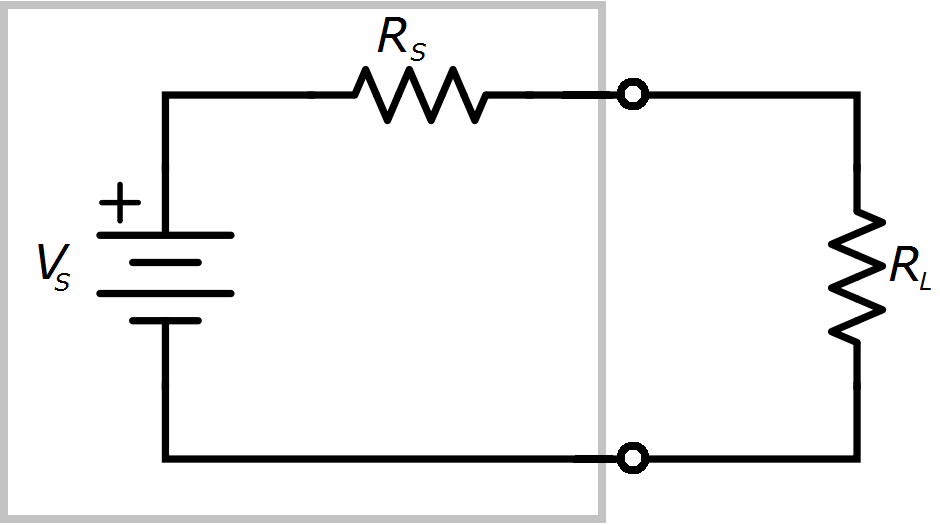
\includegraphics[width=13cm]{figures/maxPLoadMatching.png}
\caption{The simplest circuit for powering a load.}
\label{maxPowerLoadMatching}
\end{figure}
\par
The defining values for \textit{all} of the elements in the circuit of Figure \ref{maxPowerLoadMatching}---the internal voltage, internal resistance, \textit{and} the load resistance---will determine how much power is delivered to the load resistor. If the voltage is increased, it is clear that the power delivered to the load would also increase. However, assuming the voltage source is constant, what we really want to determine is how much power can be delivered to $R_L$ given the value of $R_s$.
\section{The Maximum Power Transfer Theorem}
Let's start our investigation using the voltage divider rule. $R_s$ and $R_L$ comprise a voltage divider, with $V_s$ applied across them both in series. The voltage across $R_L$ (which I will call $V_L$) is determined in the following way:
$$
V_L = V_s \cdot \left(\frac{R_L}{R_L + R_s}\right)
$$
Regardless of the values for $R_L$ and $R_s$, this expression is accurate. What we are most interested in is the power dissipated by $R_L$, and we can use one of the forms of Watt's Law in combination with this definition for $V_L$ to express the power provided to the load as 
$$
P_L = \frac{V_L^2}{R_L} = V_s^2 \cdot \left(\frac{R_L^{\bcancel{2}}}{(R_L + R_s)^2 \cdot \bcancel{R_L}}\right) = V_s^2 \cdot \left(\frac{R_L}{(R_L + R_s)^2}\right)
$$
\par
Now that we have an expression for power delivered to the load in terms of the internal circuit resistance $R_s$ and the load resistance $R_L$, we need to determine what configuration of these resistances will maximize the expression. This is an area where derivatives will come in handy! The derivative of the expression for $P_L$ with respect to $R_L$ is the slope of the function as we vary the value of $R_L$.
\begin{figure}[h!]
\centering
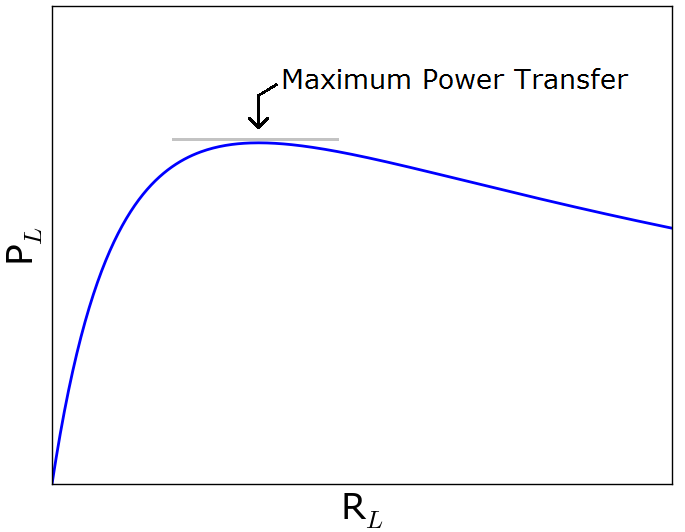
\includegraphics[width=13cm]{figures/PLvsRLrev1.png}
\caption{The shape of $P_L$ as a function of $R_L$. Maximum power is transferred to the load at the marked peak of the function.}
\label{PLvsRL}
\end{figure}
A sketch of the shape of $P_L(R_L)$ is shown in Figure \ref{PLvsRL}, and from it we can clearly see that there is a peak value. The function therefore has a derivative that passes through zero, and the specific argument used in the derivative that yields a result of zero will give the maximum value for the function itself. We're going to use that logic to find the \textit{value} for $R_L$ that maximizes power delivered \textit{to} $R_L$. 
\par
Concisely, we're going to 
\begin{enumerate}
\item{Take the derivative of $P_L$ with respect to $R_L$}
\item{Set the derivative equal to zero}
\item{Solve that equation for the value of $R_L$}
\end{enumerate}
So, taking the derivative of $P_L$ with respect to $R_L$ yields
$$
\frac{\mathrm{d}{P_L}}{\mathrm{d}R_L} = V_s^2 \cdot \frac{R_s^2-R_L^2}{(R_L + R_s)^4}
$$
\par
If we require that derivative to be zero and solve for the value of $R_L$ in that case, we find that $R_L=R_s$. This is the crux of the \textbf{Maximum Power Transfer Theorem}, which states that the maximum possible power will be transferred by the circuit to the load if the resistance of that load is equal to the internal resistance of the driving circuit. A major implication of this is that only half of the power dissipated by a circuit (at most!) can be transferred to a load.

\section{Thevenin and Norton Equivalent Circuits}
The behavior of any circuit that drives a specific load resistance ($R_L$) can be fully described by the current it causes to flow through the load and by the voltage it presents across that load. Any two circuits that provide the same current and voltage conditions to a load resistance can be described as \textbf{equivalent circuits}. Consider Figure \ref{blackboxDrivingCircuit}. The diagram on the left shows a load resistor being powered by an unknown driving circuit. For the purposes of determining power consumption by the load, the only circuit characteristics that matter are the current flowing through the load resistor and the voltage across that load. The circuits on the right of Figure \ref{blackboxDrivingCircuit} are each comprised of just two elements, but when the values of those elements are set appropriately, either of those circuits can produce the behavior of \textit{any} driving circuit for a load resistance. These two circuit types are named for their inventors---a voltage supply in series with a resistor is known as a \textbf{Thevenin equivalent circuit}, and a current supply in parallel with a resistor is known as a \textbf{Norton equivalent circuit}. 
\begin{figure}[h!]
\centering
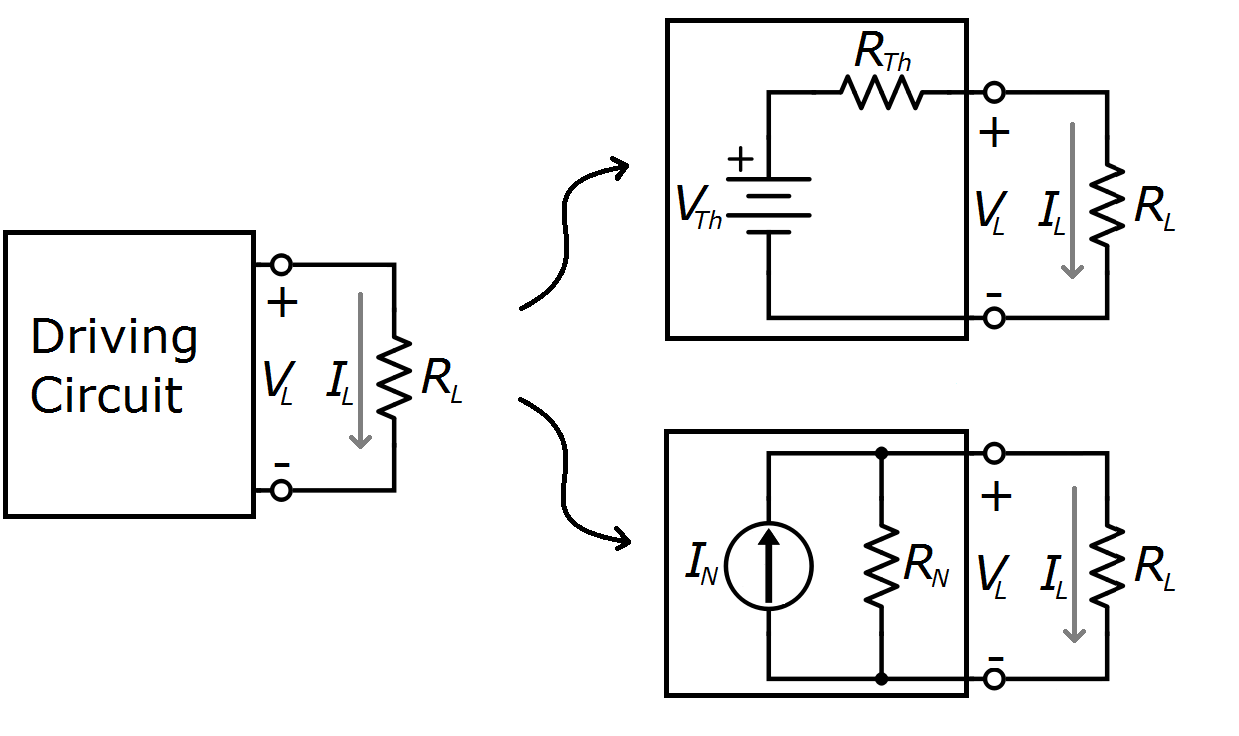
\includegraphics[width=13cm]{figures/blackboxDrivingToEquivalents.png}
\caption{The effect of a circuit on a load is described by the current flowing through that load and the voltage across the load. Regardless of the complexity of the actual driving circuit, the voltage and current characteristics of the driving circuit can be reproduced by either a voltage source in series with a resistor, or a current source in parallel with a resistor.}
\label{blackboxDrivingCircuit}
\end{figure}
\par
Like the resistor combination rules we learned in Chapter \ref{chap:resistorRulesAndTricks}, both of those equivalent circuit types can be used in the process of reducing larger circuits to smaller equivalent circuits. By recognizing that even in a larger circuit we can transform a voltage source in series with a resistor into a current source in parallel with a resistor and vice versa, we are empowered to perform these transformations while combining resistances in series and parallel to ultimately determine a single Norton or Thevenin equivalent circuit as ``seen'' by a load resistance in the larger circuit. Also, this process of transformation is quite simple. 
\par
To transform a Thevenin equivalent circuit into its corresponding Norton equivalent circuit, we need to determine how the Thevenin voltage and Thevenin resistance are related to the Norton current and Norton resistance. These releationships can be deduced from two quantities---the voltage across the two terminals where the element was connected to the circuit, and the current that would flow through a wire connecting those two terminals. These quantities are often referred to as the open-circuit voltage ($V_{oc}$) and the short-circuit current ($i_{sc}$), which are both represented in Figure \ref{ThevToNortFromOC_SC}. 
\begin{figure}[h!]
\centering
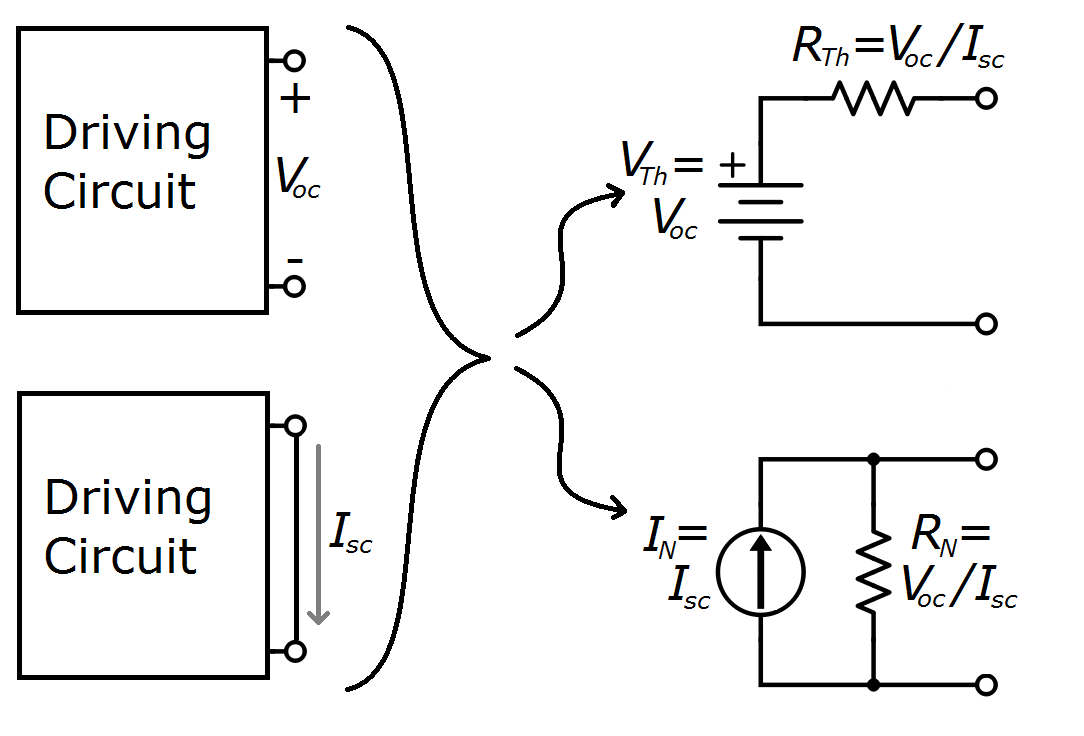
\includegraphics[width=10cm]{figures/thevNortFromOC_SC.png}
\caption{Given the open circuit voltage and closed circuit current between the two driving circuit terminals to which the load is connected, we can easily construct either a Thevenin or Norton equivalent circuit for the driving circuit. The equivalent resistance is the same for both the Thevenin and the Norton circuit.}
\label{ThevToNortFromOC_SC}
\end{figure}
With those quantities in hand, we can solve for the equivalent resistance and either the Thevenin equivalent voltage or the Norton equivalent current. The equivalent resistance is the same for either circuit:
$$
R_{Th} = R_{N} = \frac{V_{oc}}{i_{sc}}
$$
$$
V_{Th} = V_{oc}
$$
$$
i_{N} = i_{sc}
$$

These expressions confirm that converting from a Norton equivalent circuit to a Thevenin equivalent circuit and vice versa is easy. By doing so, we can simplify any resistive circuit that drives a load to its Norton or Thevenin equivalent by combining elements step by step.
\par
Let's put all this information to good use by determining the Thevenin and Norton equivalent circuits that the 1k$\Omega$ resistor in the circuit of Figure \ref{NortonTheveninEx1} ``sees'' by using the equivalent resistance combination tricks we learned in Chapter \ref{chap:resistorRulesAndTricks} in combination with the process of converting Thevenin circuits to Norton circuits and vice versa.
\begin{figure}[h!]
\centering
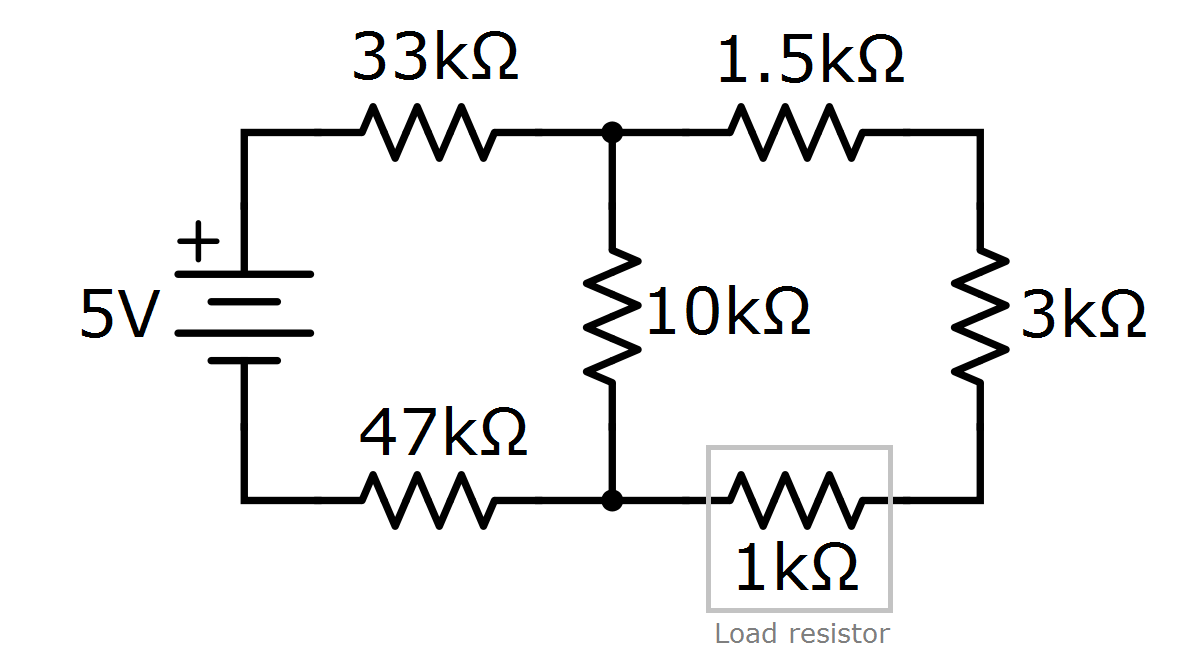
\includegraphics[width=15cm]{figures/nortThevEx_1.png}
\caption{A resistive circuit. For this example, we treat the 1k$\Omega$ resistor as the load.}
\label{NortonTheveninEx1}
\end{figure}
First, we want to take out the 1k$\Omega$ resistor, and leave open terminals at its position in the circuit. Then, we can begin simplifying the rest of the circuit that is connected to those terminals. In order to keep track of where those terminals are, it helps to redraw the remaining circuit before we continue, as shown in Figure \ref{NortonTheveninEx2}. Now, we are ready to simplify what is inside the gray box of this figure. 
\begin{figure}[h!]
\centering
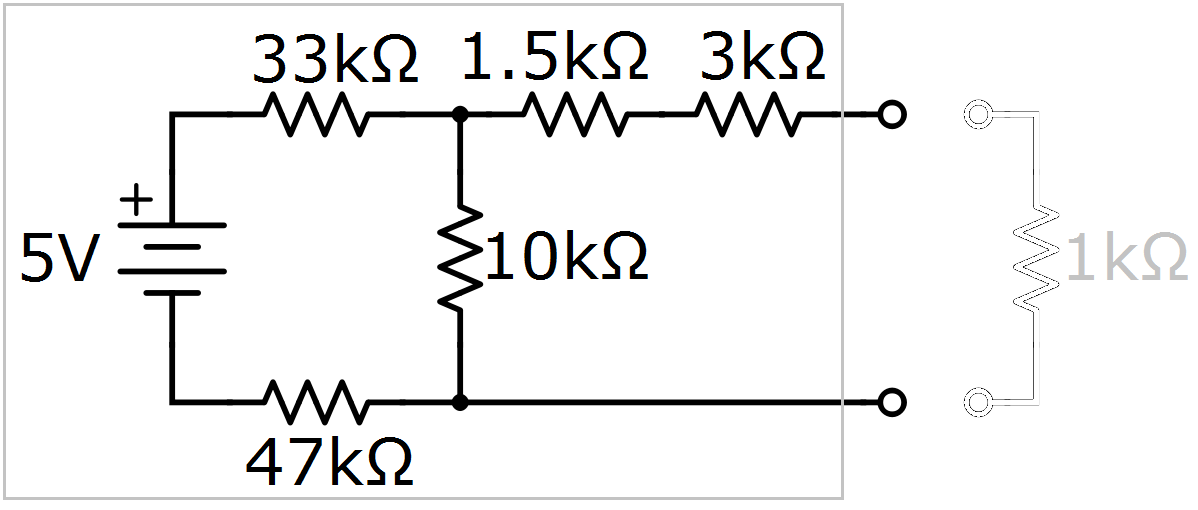
\includegraphics[width=15cm]{figures/nortThevEx_2.png}
\caption{With the 1k$\Omega$ load removed from the circuit, we simplify what is left while preserving the terminals for the load resistor.}
\label{NortonTheveninEx2}
\end{figure}
\par
Let's start by combining the 1.5k$\Omega$ and the 3k$\Omega$ resistors into an equivalent resistance of 4.5k$\Omega$ as shown in Figure \ref{NortonTheveninEx3}. At this point, there are no more obvious series or parallel resistors to combine, but if we look at the far left of the circuit, we see a 33k$\Omega$ resistor, a 47k$\Omega$ resistor, and a voltage source all in series. We can deduce that the Thevenin equivalent configuration of those three elements is a 5V source in series with a single 80k$\Omega$ resistor, as shown in Figure \ref{NortonTheveninEx4}.
\begin{figure}[h!]
\centering
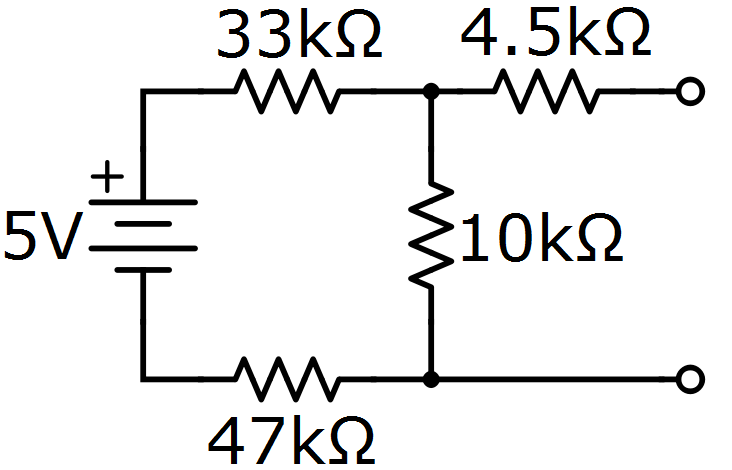
\includegraphics[width=10cm]{figures/nortThevEx_3.png}
\caption{The driving circuit after combining the series 1.5k$\Omega$ and 3k$\Omega$ resistors.}
\label{NortonTheveninEx3}
\end{figure}

\begin{figure}[h!]
\centering
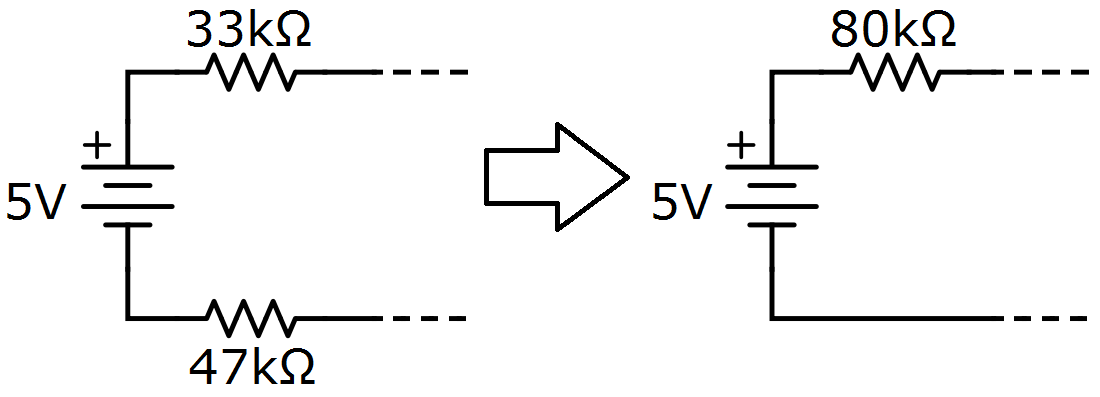
\includegraphics[width=15cm]{figures/nortThevEx_4.png}
\caption{The voltage source and two resistors at the far left of the circuit can be reconfigured as a Thevenin equivalent circuit as shown here.}
\label{NortonTheveninEx4}
\end{figure}
\par
Having found this Thevenin equivalent circuit, we can transform it into a Norton equivalent with a 62.5mA Norton current source (because 5V/80k$\Omega$=62.5mA) in parallel with an 80k$\Omega$ resistance. The resulting circuit is shown in Figure \ref{NortonTheveninEx5}. Note that now the 80k$\Omega$ and 10k$\Omega$ resistors are in parallel, and we can therefore combine them into a single 8.9k$\Omega$ resistance as shown in Figure \ref{NortonTheveninEx6}.
\begin{figure}[h!]
\centering
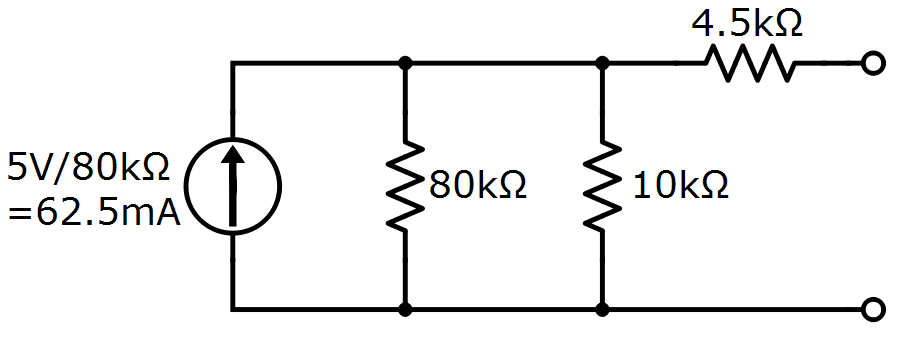
\includegraphics[width=15cm]{figures/nortThevEx_5.png}
\caption{After transforming the Thevenin equivalent circuit to a Norton equivalent, we see that the 80k$\Omega$ and 10k$\Omega$ resistors in the resulting circuit are in parallel.}
\label{NortonTheveninEx5}
\end{figure}

\begin{figure}[h!]
\centering
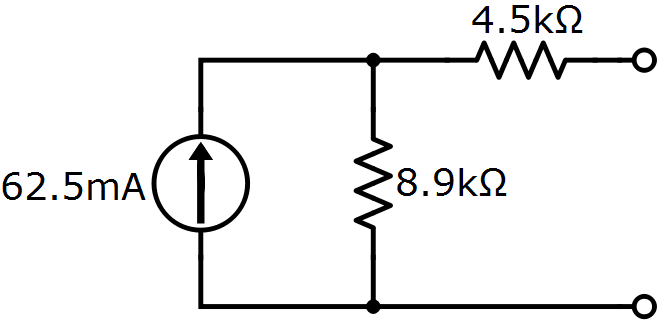
\includegraphics[width=10cm]{figures/nortThevEx_6.png}
\caption{The 80k$\Omega$ and 10k$\Omega$ resistors have been combined.}
\label{NortonTheveninEx6}
\end{figure}
\par
At this point, we've managed to pare our initial driving circuit down to just two resistors and one current source. Let's insert a Thevenin equivalent representation in place of the Norton circuit comprised of the 62.5mA current source and the 8.9k$\Omega$ resistor. That Thevenin equivalent has a voltage of 0.56V as shown in Figure \ref{NortonTheveninEx7}. The last simplification step to finding the Thevenin equivalent circuit as seen by the 1k$\Omega$ resistor is to replace the 8.9k$\Omega$ and 4.5k$\Omega$ resistors with a single 13.4k$\Omega$ resistor. The resulting Thevenin equivalent and Norton equivalent circuits are shown in Figure \ref{NortonTheveninEx8}.
\begin{figure}[h!]
\centering
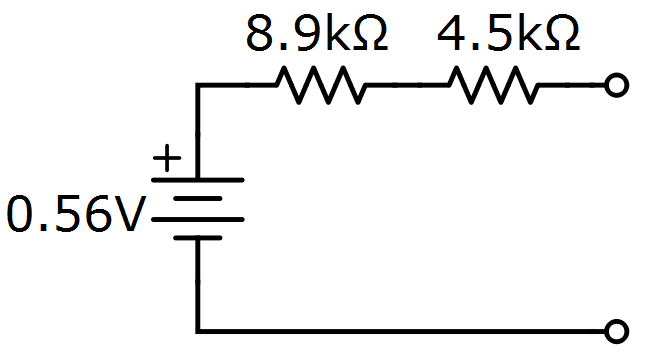
\includegraphics[width=10cm]{figures/nortThevEx_7.png}
\caption{The 62.5mA current source in parallel with the 8.9k$\Omega$ resistor (a Norton circuit) have been transformed into their Thevenin equivalent circuit.}
\label{NortonTheveninEx7}
\end{figure}

\begin{figure}[h!]
\centering
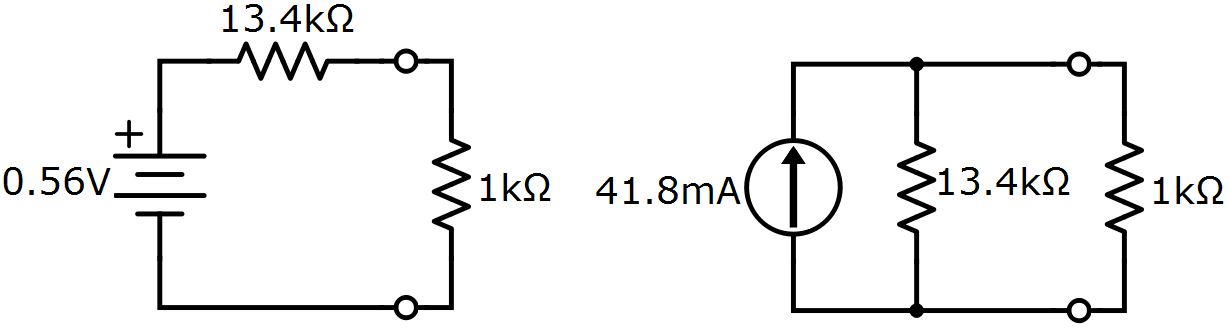
\includegraphics[width=15cm]{figures/nortThevEx_8.png}
\caption{After combining the 8.9k$\Omega$ and 4.5k$\Omega$ series resistors, the internal  resistance for the driving circuit has been found to be 13.4k$\Omega$. The Thevenin and Norton equivalent circuits as ``seen'' by the 1k$\Omega$ load resistance are shown here.}
\label{NortonTheveninEx8}
\end{figure}
\par
At this point, we can clearly see that this circuit does not deliver the maximum amount of power possible to the 1k$\Omega$ load, because the internal resistance of the circuit is 13.4k$\Omega$ rather than 1k$\Omega$. While the internal resistance of the initial circuit of Figure \ref{NortonTheveninEx1} was not obvious, reducing driving circuits to their Thevenin and Norton equivalent representations like we have done in this example makes it easy to determine what value of load resistance would maximize power delivery. 

\section{Recap: Maximum Power Transfer Theorem}
In this chapter, we learned that every circuit that drives a load resistance has an internal resistance. Even real power supplies have internal resistance. This internal resistance ties together the concepts we learned about in this chapter, namely
\begin{description}
\item[Load:] An element in a circuit for which that circuit was designed to provide power.
\item[Driving Circuit:] A circuit that is designed to power a load.
\item[Maximum Power Transfer Theorem:] The maximum possible power that a driving circuit can provide to a load will only be transferred by the circuit to the load if the resistance of that load is equal to the internal resistance of the driving circuit. Therefore, the efficiency of power delivery in electric circuits can be at most 50$\%$.
\item[Equivalent Circuits:] Equivalent circuits are circuits that provide the same voltage across and current through a load resistance. 
\item[Thevenin Equivalent Circuit:] A Thevenin equivalent circuit is comprised of just one voltage source in series with just one resistance. No matter how complicated the actual driving circuit, a Thevenin equivalent circuit can emulate the current and voltage conditions experienced by a load resistance. 
\item[Norton Equivalent Circuit:] A Norton equivalent circuit is comprised of just one current source in parallel with just one resistance. No matter how complicated the actual driving circuit, a Norton equivalent circuit can emulate the current and voltage conditions experienced by a load resistance. 
\end{description}

\chapter{Physical Properties of Capacitors and Inductors}
\label{chap:capInductorProperties}
So far we've looked at circuits with resistors, DC voltage supplies, and DC current supplies. We are about to dive into AC (time-varying) power sources, but before we do, we need to discuss two other passive elements besides resistors---the capacitor and the inductor. These circuit elements aren't very interesting in DC circuits, but they really shine when driven by AC sources. The capacitor and inductor set up internal electric and magnetic fields, respectively, when they are driven by a source that varies with time. Those fields store energy briefly rather than dissipating it away in the form of heat like resistors do. Capacitors and inductors are found in almost any electronic product you can buy today. Let's look at the physical properties of these two elements before we dig deeper and investigate their behavior in an AC circuit.
\section{Capacitor Geometry and Behavior}
\label{sec:capGeometryAndBehavior}
\begin{figure}[h!]
\centering
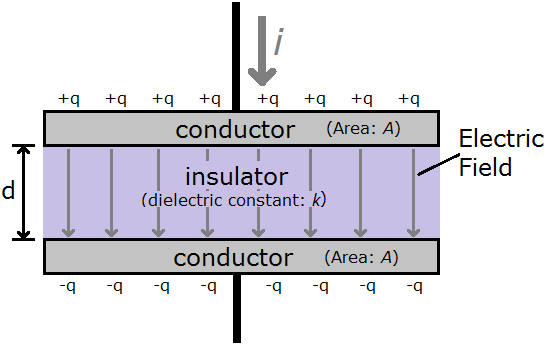
\includegraphics[width=10cm]{figures/capacitorAnnotated.png}
\caption{A capacitor is comprised of conductive plates separated by a dielectric (insulating) material. This allows an electric field to form between the plates, which is the mechanism by which a capacitor stores energy.}
\label{capInDetail}
\end{figure}
A capacitor is a circuit element that stores energy in the form of an electric field. The geometry of a capacitor is very simple; typically, a capacitor is comprised of two conductive plates separated by a layer of dielectric material. A diagram of such a device is shown in Figure \ref{capInDetail}. When a voltage source is applied across the device, electrons in the device are pulled toward the higher voltage plate of the capacitor. However, because there is not a conductive path between the plates, the higher-voltage plate builds up a net positive charge as its electrons are drawn to the positive terminal of the voltage source, and the lower voltage plate builds up a net negative charge as electrons pool there. The build-up of charge in a capacitor is related to the voltage across the capacitor according to the following expression:
$$
Q_c = C \cdot V_c
$$
When the voltage $V_c$ is built up across the plates, each plate has built up a charge of magnitude $Q_c$, but the higher voltage plate has charge of $+Q_c$, while the lower voltage plate has charge of $-Q_c$. This charge differential causes an electric field to form within the dielectric layer of the capacitor. The magnitude of this charge differential cannot grow indefinitely; eventually, the voltage of each of the plates of the capacitor will match those of the applied source, and current will cease to flow into and out of the device. 
\par
You can think of the \textbf{capacitance} for a device as a measure of how effective that device is at storing energy. The value for capacitance is based largely on the geometry of the device:
$$
C = \frac{k \cdot \epsilon_0 \cdot A}{d}
$$
In this definition, $k$ represents the \textit{dielectric constant} for the insulator material between the plates, $\epsilon_0$ is the \textit{electric permittivity of vacuum} ($8.85 \cdot 10^{-12}$F/m), $A$ is the area of each plate in the capacitor, and $d$ is the distance separating the plates. 
\par
Electric permittivity sounds really esoteric and complicated, but it's just a measure of how much charge must be built up across a medium to sustain a particular electric field. Ok, after having written that, I realize that electric permittivity \textit{is} a bit esoteric. Think about it this way: any molecule or atom can have its positively-charged nucleus and negatively-charged electron cloud pulled in opposite directions by an electric field. When that happens, the polarized atom or molecule works \textit{against} the electric field. Now, think about having a polarizable medium in between the plates of a capacitor. When voltage is applied across the capacitor and charge builds up on the capacitor plates, that forms an electric field between the plates. The medium between the plates is then polarized by the electric field, which works against the buildup of the field. Therefore, more charge is needed at the capacitor plates to create the electric field required by the applied voltage. 
\par
In contrast, vacuum has no particles to be polarized by an applied electric field. Because of that, the charge differential on the plates of the capacitor wouldn't have to fight any polarization of the vacuum in building up an electric field and such a capacitor would require \textit{less} charge across the plates to sustain a particular applied voltage. For this reason, vacuum has the lowest permittivity of any medium, and $\epsilon_0$ is used as a reference permittivity for other materials. In fact, the \textit{dielectric constant} ($k$) in the formula for capacitance above is a parameter that describes \textit{how many times larger} the permittivity of the dielectric layer material is than the permittivity of vacuum. When $\epsilon_0$ is multiplied by $k$, the result is the permittivity of the particular insulator material between the plates of the capacitor.
\par
The area and separation of the capacitor plates---$A$ and $d$, respectively---are purely spatial characteristics of the capacitor, as shown in Figure \ref{capInDetail}. We can increase capacitance by either decreasing the distance between the plates or increasing the area of the plates. In so doing, we would increase the total electric field strength in the dielectric, and thus increase the energy storage capacity for the device. We won't spend a lot of time analyzing the transient behavior of capacitors in this class, but the concepts of this section are good to keep in mind as we discuss the behavior of capacitors in circuits with AC (sinusoidally-varying) sources.
\par
Capacitance is measured in \textit{Farads} (F), which are very large units. In practice, it is most common to see capacitors within the range of picofarads ($10^{-12}$F) to hundreds of microfarads ($\sim100 \cdot 10^{-6}$F), and very uncommon to see capacitors of millifarad ($10^{-3}$F) capacitance or more.

\section{Inductor Geometry and Behavior}
\begin{figure}[h!]
\centering
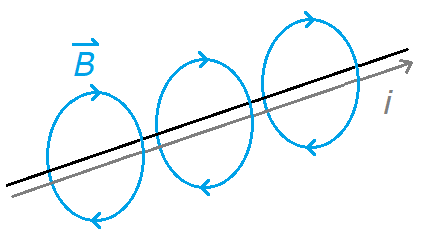
\includegraphics[width=10cm]{figures/magneticFieldInduction.png}
\caption{Current flowing through a wire ($i$) induces a magnetic field ($\vec{B}$) around that wire.}
\label{magneticFieldAroundWire}
\end{figure}

When current flows through a wire, a magnetic field is generated which curls around the wire as represented in Figure \ref{magneticFieldAroundWire}. If the wire is itself coiled, the magnetic field induced by the current flowing through the wire can reinforce itself, which is the principle by which inductors operate.
\begin{figure}[h!]
\centering
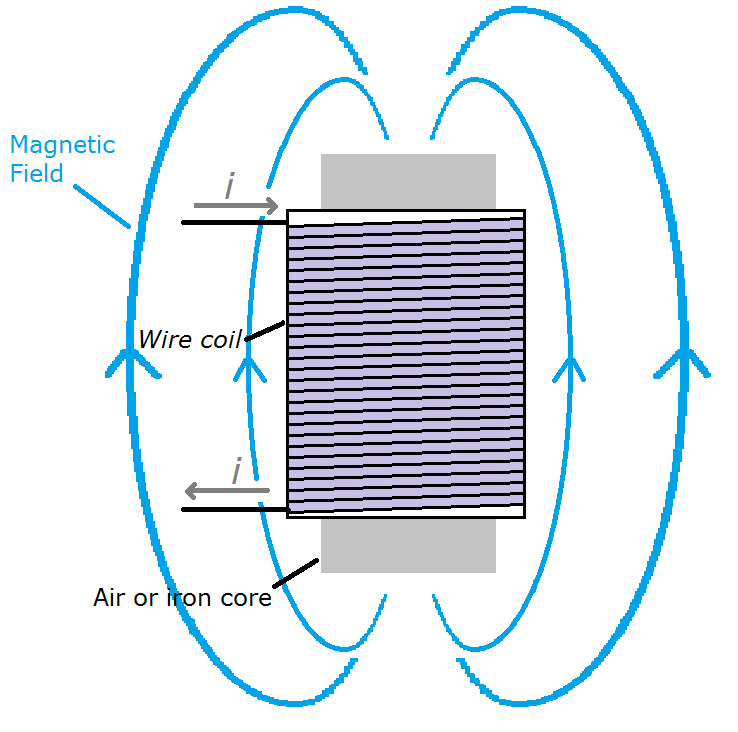
\includegraphics[width=10cm]{figures/inductorAnnotated.png}
\caption{An inductor is made of a coil of wire wrapped around a core made of air, iron, or other material. When current flows through the wire in the coil, it generates a magnetic field as indicated by the field lines in this diagram. The inductor stores energy in this field.}
\label{inductorInDetail}
\end{figure}
An inductor is simply a coil of wire wrapped around an air or iron core. When current flows through the inductor, it generates a magnetic field directed axially through the core. The \textit{magnetic flux} ($\Phi$) in the core of the inductor is defined as follows:
$$
\Phi = |\mathbf{B}| \cdot A
$$
In this definition, $|\mathbf{B}|$ is the magnitude of the magnetic field in the core, and $A$ is the cross-sectional area of the core. This flux is just part of what defines the \textbf{inductance}(L) of the device:
$$
L = N\cdot\frac{\mathnormal{d}\Phi}{\mathnormal{d}i_L}
$$
$N$ is the number of turns of wire in the inductor, $\Phi$ is the magnetic flux in the core, and $i_L$ is the current flowing through the inductor. Inductance is measured in Henries (H). In contrast to Farads, Henries are a practically-sized unit, and inductances on the order of single Henries are often encountered in practice.
\par
The physical behavior of inductors is not as easy to visualize as that of capacitors, but inductors store energy in their current-induced magnetic field. As the magnetic field in the coil of an inductor is building up or diminishing, a voltage difference across the inductor forms to counteract the change in the field. So, when there is no field inside the coil, energy is required to overcome the reactive voltage and build up the field. Conversely, once the field is present, any change in its amplitude causes another reactive voltage to form, which counteracts the change. This voltage puts energy back into the circuit from the field inside the inductor coil. If this is confusing, just remember that the field stores energy and it releases that energy back to the circuit in the form of voltage across the inductor. We will define the current-voltage relationships for the inductor and the capacitor later in this chapter.

\section{Steady-State Behavior of Capacitors and Inductors in Circuits}
In the previous section, we saw that the geometries of the capacitor and the inductor are really simple. Furthermore, if we didn't have electric or magnetic fields to consider, they would behave really simply, too. In this section, we are going to investigate the steady-state (DC) behavior of these devices in order to enhance our conceptual understanding of their behavior under eventually more dynamic conditions. 
\begin{figure}[h!]
\centering
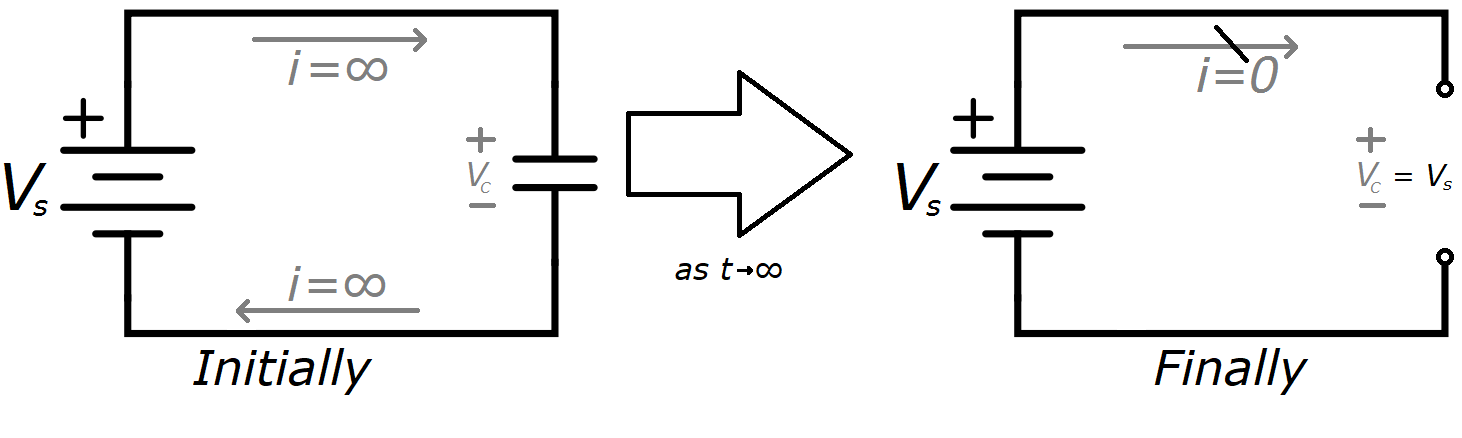
\includegraphics[width=13cm]{figures/capAndVoltage.png}
\caption{This circuit has just a voltage source and a capacitor---which is schematically represented as two unconnected parallel lines. At the moment when a voltage is applied across a capacitor, infinite current will flow into and out of the capacitor plates. This current will quickly decay as the capacitor voltage $C_V$ approaches the applied voltage $V_s$. Eventually, the capacitor acts as an open circuit with no current flowing in or out.}
\label{capSteadyState}
\end{figure}
\par
Let's consider the capacitor again for a moment. It has two disconnected conductive plates. By design, there is no path between them through which current can flow. However, when a voltage is applied across the capacitor, an initially very large current begins to flow which causes electrons to build up on the negative plate while other electrons are pulled off of the positive plate. This buildup of charge creates an electric field within the capacitor which resists further charge buildup. Because of this, the amplitude of the current flowing into and out of the capacitor decays rapidly as the voltage across the capacitor approaches the applied voltage value. Once the voltage across the capacitor reaches the value of the applied voltage, there is no more electron drift in the device, and it then acts as a simple open circuit. Figure \ref{capSteadyState} shows a diagram of this behavior. 
\begin{figure}[h!]
\centering
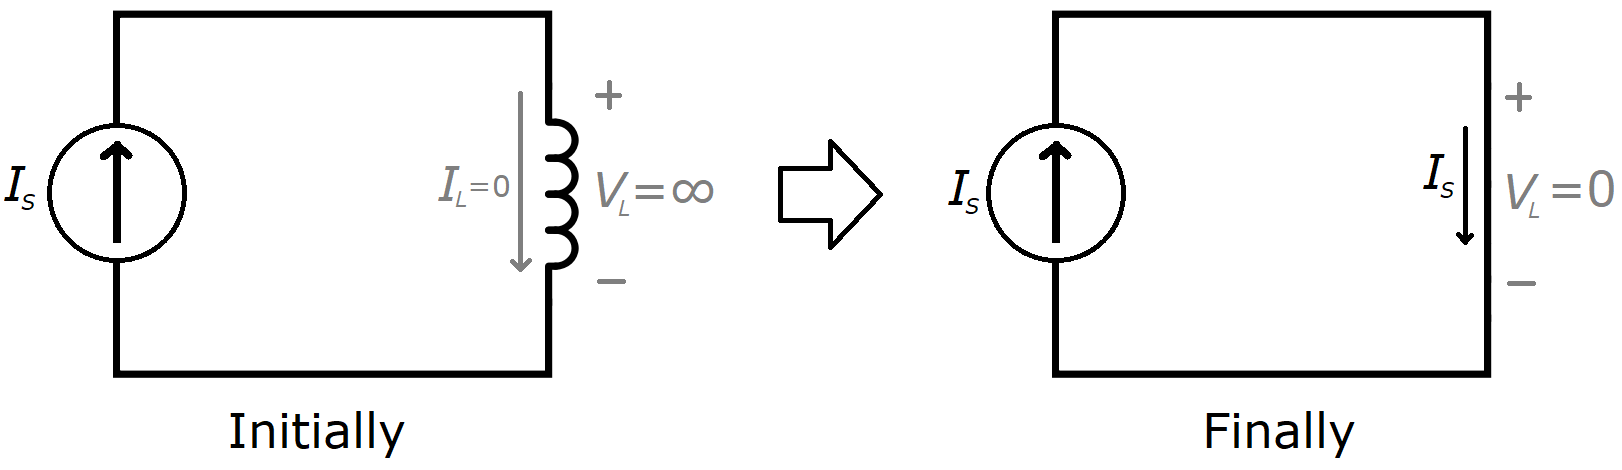
\includegraphics[width=13cm]{figures/inductorAndCurrent.png}
\caption{At the moment when a current is applied through an inductor, a very large reactive voltage forms across that inductor. However, as the inductor current approaches the applied current, the voltage across the inductor decays to zero, and then the inductor behaves like a wire.}
\label{inductorSteadyState}
\end{figure}
\par
The inductor, similarly, has very boring long-term steady-state behavior. As shown in Figure \ref{inductorSteadyState}, when a current is applied through the inductor, a very large voltage forms across the inductor in reaction to the current-induced magnetic field in the device. Initially, the current through the inductor is zero, but as it approaches the value of the applied current source, the magnitude of the magnetic field becomes stable and the voltage across the inductor diminishes to zero. Essentially, the inductor behaves just like a short circuit (i.e., a wire) once the magnetic field in the device stabilizes.
\begin{figure}[h!]
\centering
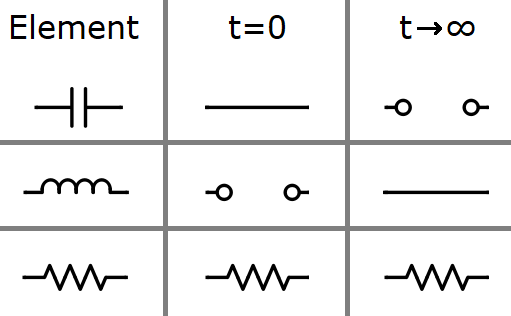
\includegraphics[width=10cm]{figures/RLClongTerm.png}
\caption{This table shows the behavior of all three passive circuit elements at the moment they are connected to a source, and after a long time has passed.}
\label{RLClongTerm}
\end{figure}
\par
To sum up the information of this section, the table in Figure \ref{RLClongTerm} concisely shows the initial and final behavior of all three passive circuit elements when they are connected to a DC power supply. The capacitor initially acts like a short circuit, but it behaves like an open circuit after some time. The inductor acts like an open circuit at first, but after some time it acts like a short circuit. And the resistor...just acts like a resistor at all times.

\section{Combining Inductors and Capacitors in Parallel and Series Configurations}
When multiple capacitors or multiple inductors are combined in one circuit, we can use some simple rules to determine an equivalent capacitance or inductance for the configuration. Let's start with inductors. If two or more inductors are in series, the equivalent inductance of the collection is the sum of all of the individual inductances. This makes sense given what we know about the geometry of an inductor; by putting multiple inductors in series with each other, we effectively increase the number of turns through which the magnetic flux passes. Also, if two or more inductors are connected in parallel, the total current flowing into them is split between the two inductors, which effectively reduces their equivalent inductance. Concisely:
$$
\textnormal{For }m\textnormal{ inductors in series:   }L_{eq} = \displaystyle\sum_{i=1}^mL_i
$$

$$
\textnormal{For }m\textnormal{ inductors in parallel:   }L_{eq} = \frac{1}{\displaystyle\sum_{i=1}^m\left(\frac{1}{L_i}\right)}
$$
\par
For capacitors, the rules are flipped; when multiple capacitors are combined in parallel, their equivalent capacitance is given by the sum of their individual capacitances. This makes sense if we think of adding a capacitor in parallel as adding surface area to the plates of a single capacitor. According to the equation for capacitance we saw in Section \ref{sec:capGeometryAndBehavior}, the capacitance increases with the area of the plates. If multiple capacitors are in series, however, the effective separation between their plates is equal to the sum of all the plate separations. This spreads the electric field out over a larger distance, and therefore the equivalent capacitance is less than the individual capacitances in the series. The rules for combining capacitances are:
$$
\textnormal{For }m\textnormal{ capacitors in parallel:   }C_{eq} = \displaystyle\sum_{i=1}^mC_i
$$
$$
\textnormal{For }m\textnormal{ capacitors in series:   }C_{eq} = \frac{1}{\displaystyle\sum_{i=1}^m\left(\frac{1}{C_i}\right)}
$$
\section{Derivation of the Voltage-Current Relationship for Capacitors and Inductors}
\textbf{Warning: calculus ahead.} The point of this section is to figure out how to relate current flowing through and voltage across both capacitors and inductors. If I use V = i $\times$Z (Ohm's Law) to do this, what is Z for capacitors and inductors? I answer that question in this section.
\par
To use the rules we learned about in Chapters \ref{chap:fundamentals} and \ref{chap:resistorRulesAndTricks} to analyze capacitor and inductor circuits, we need to be able to relate voltage across capacitors and inductors to current flowing through them. The mathematical expressions relating the physical relationships between current and voltage for both the capacitor and the inductor are, unfortunately, differential equations. For example, the current flowing into and out of a capacitor defines the change of voltage across that capacitor in the following way:
$$
i_C(t) = C \cdot \frac{d}{dt}V_C(t)
$$
Gross. However, we can define the capacitor and inductor impedances in a time-independent way as long as we assume the time-dependence of the driving source is sinusoidal with a single driving frequency. This may initially seem overly restrictive and possibly useless in practice, but as you will learn in your math classes if you haven't already, any time-varying signal can be represented as a linear superposition of sinusoids. Therefore, if we know how to characterize the impedance of a capacitor or inductor for a sinusoidal driving source with a single frequency, we could characterize the impedance of these elements for any range of frequencies.
\par
Let's manipulate the equation above until we are able to solve for $V_C/i_C$. This ratio is called the \textbf{impedance} of the capacitor, and it is represented by $Z_C$. (Ohm's Law is actually defined in terms of impedance as $V=i\times Z$, but we will discuss this more in the next chapter.)
\par
Let's first assume that 
$$
V_C(t) = V_0\cos(\omega t)
$$
and therefore 
$$
\frac{d}{dt}V_C(t)=-\omega V_0 \sin(\omega t)
$$
Combining these expressions yields the following:
$$
i_C(t) = C \cdot \left(-\omega V_0 \sin(\omega t)\right)
$$
Recall\footnote{As a student, I always used to love it when textbook authors would tell me to recall things I often hadn't ever heard before. If you find yourself in that position here, think about it for a minute, or just take my word for it and don't worry about recalling a thing!} that $-\sin(\omega t)$ differs from $\cos(\omega t)$ only by a phase shift of $\pi/2$:
$$
-sin(\omega t) = cos(\omega t + \pi/2)
$$
Now we want to separate the cosine term from the phase. To do this we will use, \textit{Euler's Formula}:
$$
e^{j\theta} = \cos{\theta} + j\sin{\theta}
$$
This formula introduces $j$, which is defined as $\sqrt{-1}$.\footnote{Before we go any further: in electrical engineering, we use ``$j$'' to denote $\sqrt{-1}$ instead of ``$i$''. We do this because ``$i$'' already denotes current, and for other historical reasons. Regardless of why, I will be using ``$j$'' in this way from now on.} We will explore imaginary numbers in more detail in the next chapter, but according to Euler's formula, multiplying $\cos(\omega t)$ by $e^{j\pi/2}$ is one way of introducing a phase shift of $\pi/2$. Therefore, we can rewrite our expression for $i_C$ in the following way:
$$
i_C(t) = e^{j\pi/2} C \omega \left(V_0 \cos(\omega t)\right)
$$
We now have our initial form of $V_C$ back in the equation, which means we're almost ready to solve for impedance. Before we do that though, we need to do something about that exponential term. Using Euler's formula again, we find that 
$$
e^{j\pi/2} = \cancelto{0}{\cos(\pi/2)} + j\cdot\cancelto{1}{\sin(\pi/2)}=j
$$
Finally, rewriting our expression for $i_C(t)$ yields 
$$
i_C(t) = j\omega C V_C(t)
$$
Therefore, for a sinusoidal driving source of frequency $\omega$, the impedance of a capacitor is
$$
Z_C = \frac{V_C}{i_C} = \frac{1}{j\omega C}
$$
This is better, but now we've traded time-dependence for ``imaginary-ness''. Which is worse? Well, time dependence is worse, obviously, but we will need to refresh our memories concerning imaginary numbers before we can do much with this impedance.
\par
The relationship between current and voltage for an inductor is complimentary to that for a capacitor:
$$
V_L(t) = L \cdot \frac{d}{dt}i_L(t)
$$
Assuming $i_L=I_0\cos(\omega t)$, and skipping most of the steps to get here, we find that 
$$
V_L = j\omega L i_L(t)
$$
Therefore, for a sinusoidal driving source of frequency $\omega$, the impedance of an inductor is
$$
Z_L = j\omega L
$$
\par
After the next chapter reintroduces complex algebra to you, firehose style, we will use the impedances derived above extensively to analyze circuits using resistors, capacitors, and inductors.
\section{Recap: Capacitors and Inductors}
You have now seen everything you need to know (and more) about capacitors and inductors for the purposes of this course. In the following chapters, we will apply the concept of impedance to analyze some circuits and to do some simple circuit design. For now, here are the highlights of this chapter listed succinctly:
\begin{description}
\item[Capacitance:] This is a measure of the energy storage capacity that a capacitor has. $$C = \frac{k \cdot \epsilon_0 \cdot A}{d}$$ where k is the relative permittivity of the dielectric material in the capacitor, A is the area of the capacitor plates, and d is the distance between the plates.
\item[Inductance:] This is a measure of the energy storage capacity an inductor has. $$
L = N\cdot\frac{\mathnormal{d}\Phi}{\mathnormal{d}i_L}
$$ where N is the number of wire turns for the inductor, $\Phi$ is the flux of the magnetic field through the inductor, and $i_L$ is the current flowing through the inductor that creates the magnetic field.
\item[Equivalent Inductance:] The rules for combining inductors are similar to the rules for combining resistors. 
$$
\textnormal{For }m\textnormal{ inductors in series:   }L_{eq} = \displaystyle\sum_{i=1}^mL_i
$$

$$
\textnormal{For }m\textnormal{ inductors in parallel:   }L_{eq} = \frac{1}{\displaystyle\sum_{i=1}^m\left(\frac{1}{L_i}\right)}
$$

\item[Equivalent Capacitance:] The rules for combining capacitors are the opposite of the rules for combining resistors.
$$
\textnormal{For }m\textnormal{ capacitors in parallel:   }C_{eq} = \displaystyle\sum_{i=1}^mC_i
$$

$$
\textnormal{For }m\textnormal{ capacitors in series:   }C_{eq} = \frac{1}{\displaystyle\sum_{i=1}^m\left(\frac{1}{C_i}\right)}
$$

\item[Capacitor Impedance:] $Z_C = \frac{1}{j\omega C}$
\item[Inductor Impedance:] $Z_L = j\omega L$
\end{description}

\chapter{Complex Algebra and Phasor Notation}
\label{chap:complexAlgebra}
In the last chapter, I introduced the concept of \textit{impedance}, which is a complex quantity that relates the voltage across a circuit element to the current through that element. From this point on in the course, impedance will supercede resistance in our calculations of circuit behavior. For that reason, and because impedance calculations require an understanding of complex algebra, this chapter will just focus on representations of complex numbers and on rules for adding, subtracting, multiplying, and dividing them. Think of this chapter as a complex algebra-focused interlude. 

\section{Representations of Complex Numbers}
A complex number is comprised of two parts: its real part, and its imaginary part. One way to represent complex numbers is by expressing their real and imaginary parts separately. Think of this as a vector in the two-dimensional complex plane. This is called the \textbf{Cartesian} form for a complex number, because it easily maps to a Cartesian coordinate system with real numbers along the horizontal axis and imaginary numbers along the vertical axis as shown in Figure \ref{cartesianZ}. In this figure, the real and imaginary parts of Z provide the horizontal and vertical coordinates of Z in the complex plane, respectively. The Cartesian form for a generic complex number $Z$ is expressed as follows:
$$
\textbf{Cartesian form:}\textnormal{                         }Z=\underbrace{a}_{\textnormal{real part}} + \underbrace{j\cdot b}_{\textnormal{imaginary part}}
$$
\begin{figure}[h!]
\centering
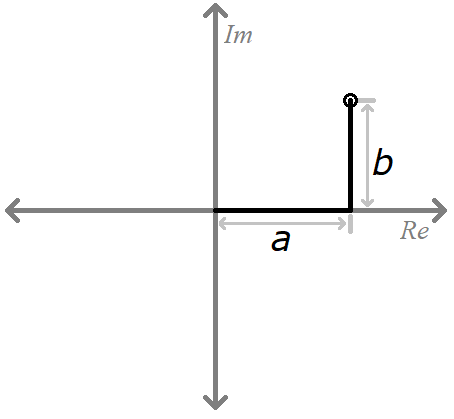
\includegraphics[width=5cm]{figures/ZCartesian.png}
\caption{The complex number Z mapped onto the complex plane using Cartesian coordinates.}
\label{cartesianZ}
\end{figure}
\par
Another way to represent complex numbers is by specifying the magnitude of the vector and a phase angle. This is called the \textbf{polar} form for a complex number, because it easily maps to a polar coordinate system in the complex plane, as shown in Figure \ref{polarZ}. The plane in this figure is still real on the horizontal axis and imaginary along the vertical axis. Now, however, the complex number is plotted by rotating counter-clockwise from the positive real axis to the specified phase angle and then plotting a line out from the origin by the specified magnitude. In other words, the magnitude and angle of Z indicate how far Z is from the origin and what angle Z sweeps out with respect to the positive real axis, respectively. 
\begin{figure}[h!]
\centering
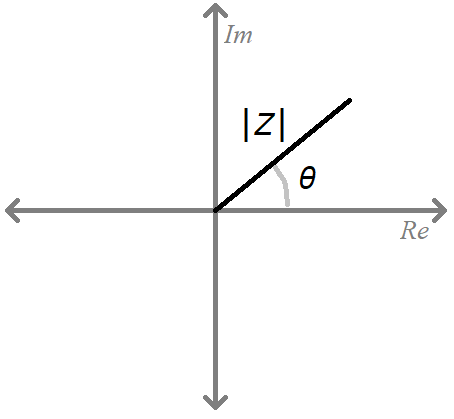
\includegraphics[width=5cm]{figures/ZPolar.png}
\caption{The complex number Z mapped onto the complex plane using Polar coordinates.}
\label{polarZ}
\end{figure}
We will often write the polar form in an abbreviated way known as the \textbf{phasor} representation of the number. The polar and phasor forms for a generic complex number are given below: 
$$
\textbf{Polar form:}\textnormal{                 } Z = |Z|e^{j\theta}
$$
$$
\textbf{Phasor form:}\textnormal{                 } Z = |Z|\angle\theta
$$
\par
As we will see in the next section, it is nice to have more than one way to represent complex numbers because some arithmetic operations are easier with one form than the other. If we ever need to convert a complex number from Cartesian form to polar form or vice versa, we can do so using the following rules:
$$
\textbf{Converting Cartesian to polar form: }a + j\cdot b = \sqrt{a^2 + b^2}e^{j(\arctan(b/a))}
$$
$$
\textbf{Converting polar to Cartesian form}\footnote{Remember Euler's formula: $e^{j\theta} = cos\theta + j sin\theta$}\textbf{: }|Z|e^{j\theta} = |Z|\cos(\theta) + j\cdot |Z|\sin(\theta)
$$


\section{Adding, Subtracting, Multiplying, and Dividing Complex Numbers}
When we add or subtract complex numbers, it is easiest to do so using their Cartesian form, because the real parts and the imaginary parts need to be added or subtracted separately from each other. If we need to add complex numbers that are in phasor or polar form, it's best to convert them to Cartesian form first. Here are the rules for addition and subtraction of complex numbers, using two generic complex numbers $Y=a+j\cdot b$ and $Z=c+j\cdot d$:
$$
(Y+Z) = (a+c) + j\cdot(b+d)
$$
$$
(Y-Z) = (a-c) + j\cdot(b-d)
$$
\par
When we multiply or divide complex numbers, it is easiest to do so using their polar or phasor form, because this reduces the amount of tedious arithmetic we must do to obtain the result. If we need to multiply two complex numbers, we could do so using Cartesian form, but it's easiest in polar form. And, when we need to divide two complex numbers, it is best to convert both to polar or phasor form. Here are the rules for multiplication and division of complex numbers using two generic complex numbers $Y = |Y|\angle\theta$ and $Z = |Z|\angle\phi$:
$$
(Y\cdot Z) = (|Y|\cdot|Z|)\mathlarger{\angle}(\theta+\phi)
$$
$$
\left(\frac{Y}{Z}\right) = \left(\frac{|Y|}{|Z|}\right)\mathlarger{\angle}(\theta-\phi)
$$
We can also multiply two complex numbers in Cartesian form if necessary (using the F.O.I.L. method), but remember that $j\cdot j=-1$. Using two generic complex numbers $Y=a+j\cdot b$ and $Z=c+j\cdot d$:
$$
(Y\cdot Z) = (a+j\cdot b)\cdot(c+j\cdot d) = (a\cdot c) + j\cdot (b\cdot c) + j\cdot(a\cdot d) + \cancelto{-1}{j^2}\cdot (b\cdot d) 
$$
$$
= [(a\cdot c) - (b\cdot d)] + j\cdot[(b\cdot c) + (a\cdot d)]
$$
\section{Shortcuts with $j$}
Like many things in life, the main way you will get better at complex algebra is through practice using it. However the tricks in this section will save you lots of time if you remember them because they are really useful in the context of circuits, and they seem to come up often.
\par
You may sometimes find these angle-to-imaginary-number relationships useful when you are needing to convert a complex number from Cartesian to phasor form or vice versa:
$$
\angle{90^{\circ}} = \angle\left(\frac{\pi}{2}\right) = j
$$
$$
\angle{-90^{\circ}} = \angle{-\left(\frac{\pi}{2}\right)} = -j
$$
$j$ is tricky, and sometimes it shows up where it shouldn't. The following equations give you easy ways to push $j$ around.
$$
j^2 = -1
$$
$$
\frac{1}{j} = -j
$$
\section{Back to Circuits: Complex Impedance}
Remember that Ohm's law defines \textit{resistance} as the ratio of voltage across the resitor to the current flowing through that resistor. If we extend Ohm's law into the domain of complex numbers, a more general version of Ohm's law emerges:
$$
V = i \cdot Z
$$
This is not too impressive on the surface, but now in the place of a fully-\textit{real} resistance, $R$, we have a complex-valued \textbf{impedance}, $Z$. Impedance can be broken into two parts:
$$
Z = \underbrace{R}_{Resistance} + \textrm{  } j \cdot \underbrace{X}_{\mathclap{Reactance}}
$$
\par
From the above definition, we see that the resistance is the real part of impedance. We call the complex part of impedance reactance. This means that the resistance we have studied so far is a special case of the larger concept of impedance. In Chapter \ref{chap:capInductorProperties}, we derived the impedance for capacitors and inductors under sinusoidal driving conditions. Capacitor and inductor impedances are purely \textit{reactive}. Using the conversion techniques of this chapter, those impedances are represented in Cartesian and phasor form as follows:
$$
Z_C = \frac{1}{j\omega C} = \frac{-j}{\omega C} = \left(\frac{1}{\omega C}\right)\mathlarger{\mathlarger{\angle}}-\left(\frac{\pi}{2}\right)
$$
$$
Z_L = j\omega L = \omega L\mathlarger{\mathlarger{\angle}}\left(\frac{\pi}{2}\right)
$$
Now that we've covered the rules for manipulating complex numbers, we can use these expressions for impedance along with resistance to analyze AC circuit behavior.

\section{Recap: Representing and Manipulating Complex Numbers}
Complex numbers may seem obscure; anything we un-ironically refer to as ``imaginary'' really does warrant some careful explanation. However, the representations of and rules for manipulating complex numbers presented in this chapter will be very useful as we proceed with the rest of the course. This recap might come in handy as a reference.
\begin{description}
\item[Cartesian form:]
$$
Z=\underbrace{a}_{\textnormal{real part}} + \underbrace{j\cdot b}_{\textnormal{imaginary part}}
$$
\item[Polar form:]
$$
Z = |Z|e^{j\theta}
$$
\item[Phasor form:]
$$
Z = |Z|\angle\theta
$$
\item[Converting Cartesian to Polar and Phasor Form:]
$$
a + j\cdot b = \sqrt{a^2 + b^2}e^{j(\arctan(b/a))} = \sqrt{a^2 + b^2}\angle(\arctan(b/a))
$$
\item[Converting polar to Cartesian form:]
$$
|Z|e^{j\theta} = |Z|\cos(\theta) + j\cdot |Z|\sin(\theta)
$$
\item[Addition and Subtraction of Complex Numbers:] This is done in Cartesian form. Using two generic complex numbers $Y=a+j\cdot b$ and $Z=c+j\cdot d$:
$$
(Y+Z) = (a+c) + j\cdot(b+d)
$$
$$
(Y-Z) = (a-c) + j\cdot(b-d)
$$
\item[Multiplication and Division of Complex Numbers:] This is done in polar or phasor form. Using two generic complex numbers $Y = |Y|\angle\theta$ and $Z = |Z|\angle\phi$:
$$
(Y\cdot Z) = (|Y|\cdot|Z|)\mathlarger{\angle}(\theta+\phi)
$$
$$
\left(\frac{Y}{Z}\right) = \left(\frac{|Y|}{|Z|}\right)\mathlarger{\angle}(\theta-\phi)
$$
We can also multiply two complex numbers in Cartesian form. Using two generic complex numbers $Y=a+j\cdot b$ and $Z=c+j\cdot d$:
$$
(Y\cdot Z) = [(a\cdot c) - (b\cdot d)] + j\cdot[(b\cdot c) + (a\cdot d)]
$$
\item[Additional representations for $j$:] 
$$
\angle90^{\circ} = j
$$
$$
\angle-90^{\circ} = -j
$$
$$
j^2 = -1
$$
$$
\frac{1}{j} = -j
$$
\item[Impedance:] The complex ratio of voltage across to current flowing through a passive circuit element. Resistance is the \textit{real} part of impedance:
$$
Z = \underbrace{R}_{Resistance} + \textrm{  } j \cdot \underbrace{X}_{\mathclap{Reactance}}
$$



\end{description}
\chapter{Passive AC Circuit Analysis}
\label{chap:ACcircuits}
Now that we've covered complex numbers, you are ready to ``dive into'' signal processing! Well, more like ``dip your toes in''. Swimming pool analogy aside, when circuits are designed to manipulate time-varying signals, we use the complex algebra introduced in the last chapter to describe and analyze their behavior. In this chapter, we will learn how.
\section{AC Sources and their Phasor Representations}
AC circuits are driven by AC sources. Those sources are represented in a variety of ways, but the most common representations are shown in Figure \ref{ACsources}. From this figure, we see that the AC voltage symbol is distinct from the DC voltage symbols we have used. However, the AC current symbol is identical to that for DC current sources; context is required to distinguish between AC and DC current sources. 
\begin{figure}[h!]
\centering
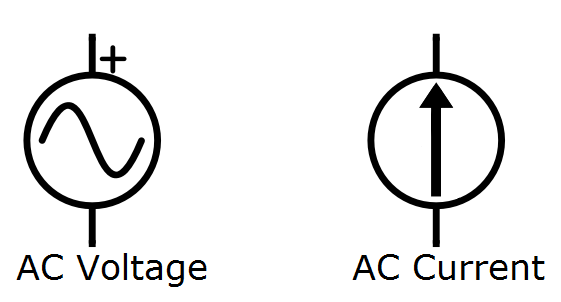
\includegraphics[width=10cm]{figures/ACsources.png}
\caption{Schematic symbols for AC sources. The voltage symbol is clearly different from that for a DC source, but the AC current symbol requires the context of a label to distinguish it from a DC current source.}
\label{ACsources}
\end{figure}
\par
When an AC source is present in a circuit, the time-dependent function of its voltage or current will often be given. When we analyze these circuits, it is always preferrable to do so in phasor notation. This allows us to rely solely on algebra and avoid the unneccesary use of differential equations.\footnote{You might like differential equations. I do, too. However, doing hard things is not what being a professional scientist or engineer is all about. Rather, it's about finding easy ways to do the hard things so you can do them faster! Also, if you take more circuits courses, you will definitely get to practice those DE skills.} So, if you are given a functional description of an AC source, you need to be able to convert that to a phasor representation.
\par
Let's assume we have an AC voltage source that provides a voltage of $V_s(t) = V_0\cos(\omega t + \theta)$. To convert this to phasor form, we need to isolate its magnitude and its phase angle. For this function, like for any cosine function, this is easy; the amplitude is $V_0$, and the phase angle is $\theta$. Therefore, conversion from time-dependent form to phasor form follows this pattern:
$$
V_s(t) = V_0\cos(\omega t + \theta) \leftrightarrow V_0\angle\theta \textnormal{ (with frequency }\omega\textnormal{)}
$$
In addition to the phasor form of our source, its frequency will still be important as we calculate the impedances of the different elements in our circuit; remember that the impedances for both a capacitor and an inductor are dependent on the driving frequency, which will always be the frequency of the AC source in the circuit. 
\par
When we are finished with circuit analysis, we will often want to express our answers in time-dependent form. So, we need to be able to convert a phasor representation into a time-dependent functional representation. To do so only requires us to reverse our steps from before. \textbf{The frequency will not change throughout this process.} 
\section{The Process of AC Circuit Analysis by Example}
Now, let's put all of these equations to work in an example. Most of this will follow what we did in DC.
\begin{figure}[h!]
\centering
\includegraphics[width=10cm]{figures/firstACcircuit.png}
\caption{An AC circuit with an AC voltage source driving a resistor, a capacitor, and an inductor in series.}
\label{myFirstACCircuit}
\end{figure}
\par
Consider the circuit of Figure \ref{myFirstACCircuit}. In this circuit, an AC voltage source is connected to an inductor, a capacitor, and a resistor in series. We need to find the time-dependent voltage across the resistor, $V_R$. To do this, we will rely on the techniques we learned in Chapters \ref{chap:fundamentals} and \ref{chap:resistorRulesAndTricks}, but we will extend them into the realm of complex impedance. But first, we must convert all the quantities given into their equivalent phasor representations.
\par
The voltage source can be represented with the phasor 5V$\angle$0, and we note that its frequency, $\omega$, is 100 rad/s. We will use that frequency to determine the impedances for the inductor and the capacitor according to the expressions for capacitor and inductor impedance from Chapter \ref{chap:capInductorProperties}:
$$
Z_C = \frac{1}{j\omega C} = \frac{1}{j\cdot100\cdot10^{-6}} \Omega= -j\cdot10^{4}\Omega
$$
$$
Z_L = j\omega L = j(100\cdot5) \Omega = j\cdot500\Omega
$$
These impedances are in Cartesian form. Before we proceed, let's also determine their equivalent phasor forms. We can use shortcuts from Chapter \ref{chap:complexAlgebra} in this conversion: $e^{j\pi/2}=j$, and ``$j$''$\rightarrow\angle\pi/2$. Similarly, $e^{-j\pi/2}=-j$, and ``$-j$''$\rightarrow\angle-\pi/2$. Therefore, 
$$
Z_C = -j\cdot10^{4}\Omega = (10^4\angle-\pi/2)\Omega
$$
$$
Z_L = j\cdot500\Omega = (500\angle\pi/2)\Omega
$$
Both of these forms might come in handy, and usually it's a good idea to have both forms available as you begin to analyze a circuit. We should also note that the resistor's impedance has Cartesian and phasor forms, too, but they are simple in comparison with those for the capacitor and inductor because the impedance of the resistor is entirely \textit{real}. Therefore, the Cartesian form for the resistor is just $1000\Omega$, and the phasor form is $(1000\angle0)\Omega$.
\par
Now that we have all the impedances calculated and the phasor representation for the source, we can redraw the circuit using these to label the respective elements, as shown in Figure \ref{myFirstACCircuit2}.
\begin{figure}[h!]
\centering
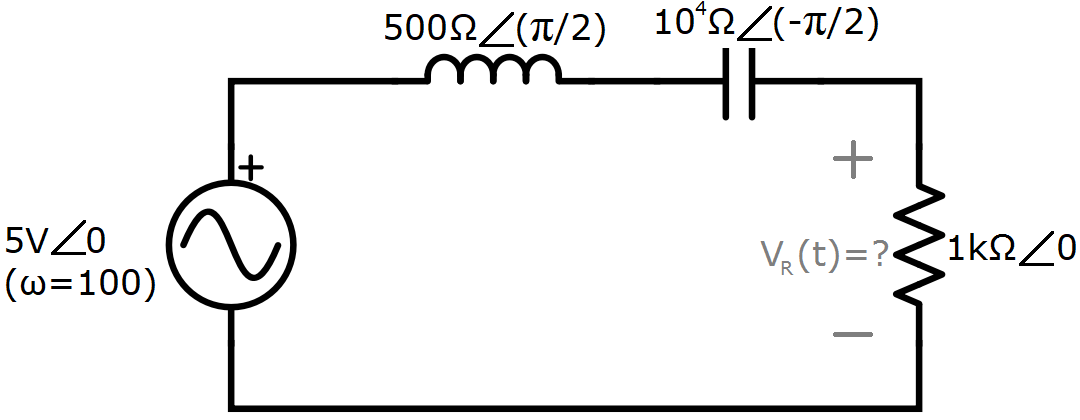
\includegraphics[width=10cm]{figures/firstACCircuit2.png}
\caption{The same circuit as before, but with the elements labeled by the phasor representations of their impedances.}
\label{myFirstACCircuit2}
\end{figure}
 Now that we have calculated the impedances for the capacitor and the inductor, we can use KVL, KCL, Ohm's Law, the Voltage Divider Rule, and the Current Divider Rule to analyze this circuit just like we did for purely resistive DC circuits! This means that if you were able to do the DC analysis in previous chapters, you already have the knowledge required to do what's coming next. 
 \par
 What we want to solve for is the time-dependent voltage across the resistor. In Chapter \ref{chap:resistorRulesAndTricks} we learned that when we have a series of resistances, we can treat those as a \textit{voltage divider}, which allows us to solve for the voltage across one element of the series without having to find the current flowing through that series of elements. This rule extends to complex impedances, which means that we can treat the series of the inductor, capacitor, and resistor as a voltage divider, too, for the purpose of determining the voltage across just the resistor. The total impedance of the series is the sum of their impedances, which is just like the rule we use to combine resistors in series, and  the voltage across the entire series is simply the AC voltage supply. Therefore, the expression for voltage across the resistor is as follows:
 $$
V_R = V_S\cdot\left(\frac{Z_R}{Z_R+Z_C+Z_L}\right)=(5V\angle0)\left(\frac{1000\angle0}{(1000 + j\cdot500 - j\cdot10^4)}\right)
$$
$$
=(5V\angle0)\left(\frac{1000\angle0}{(1000 - j\cdot9500)}\right)
 $$
Before we can finish solving for the phasor form of $V_R$, we need to convert the sum of the three impedances in the denominator from Cartesian form to phasor form. We learned how to do this in Chapter \ref{chap:complexAlgebra}:
$$
1000 - j\cdot9500 = \sqrt{1000^2+9500^2}\angle\arctan(-9500/1000) = 9552.5\angle(-1.46)
$$
Replacing the Cartesian form with this phasor allows us to complete the calculation of the phasor form for $V_R$:
$$
V_R = (5V\angle0)\left(\frac{1000\angle0}{(1000 - j\cdot9500)}\right) = (5V\angle0)\left(\frac{1000\angle0}{9552.5\angle(-1.46)}\right)
$$
$$
= (5V\angle0)\cdot\left(\left(\frac{1000}{9552.5}\right)\angle\left(0- \left(-1.46\right)\right)\right)=(5V\angle0)\cdot(0.1\angle1.46)
$$
$$
=(5\cdot0.1)\angle(0+1.46)=0.5V\angle1.46
$$
With the phasor form for the voltage across the resistor found, we only need to convert that to the time-dependent functional form to be through with this analysis. The amplitude of the voltage is 0.5V, the phase angle is 1.46 radians, and the frequency is the same as the driving frequency, which was 100 rad/s. Putting all these pieces together, we find the functional form for the time-dependent voltage across the resistor: 
$$
v_R(t)= 0.5V\cos(100\cdot t + 1.46)
$$
And that concludes our analysis!
\par
The equations we used in this example were exactly what we would have used if we only had resistors in our circuit; all the rules and tricks we used were the same, except that we were using complex impedance instead of all-real resistance. In other words, the most challenging part about AC circuit analysis as compared to DC circuit analysis is the fact that we are working with complex numbers instead of all real numbers. 
\section{Frequency-Dependent Behavior in AC Circuits}
Now that we are dealing with frequency-dependent impedances, we should examine the effects of changing our source frequency on the results of our calculations. Let's consider the example of the previous section, but let's change the source frequency from 100 rad/s to 10rad/s. Eventually, you will be able to predict the effect of such a frequency change on the voltage across the resistor, but for now, let's recalculate it.
\par
First, we need to calculate the new impedances for the inductor and capacitor. Since the source frequency is now $1/10^{th}$ its previous value, we can adjust the impedances of the inductor and the capacitor by dividing by 10 and multiplying by 10, respectively:
$$
Z_L = j\cdot50\Omega
$$
$$
Z_C = -j\cdot10^5\Omega
$$
Using these values in the above calculation of $v_R(t)$ yields the following result:
$$
V_R = (5V\angle0)\left(\frac{1000\angle0}{(1000 - j\cdot99950)}\right) = (5V\angle0)\left(\frac{1000\angle0}{99955.0\angle(-1.56)}\right)
$$
$$
= (5V\angle0)\cdot\left(\left(\frac{1000}{99955.0}\right)\angle(0- (-1.56))\right) = (5V\angle0)\cdot(0.01\angle1.56)
$$
$$
V_R=0.05V\angle1.56
$$
Therefore,
$$
v_R(t)=0.05V\cos(10\cdot t + 1.56)
$$
\par
From this result, we see that as the source frequency decreases, the amplitude of the voltage drop across the resistor decreases, too. Furthermore, the phase difference across the resistor appears to approach $\pi/2$ as the driving frequency decreases.\footnote{This makes sense, because the dominant impedance of the three passive elements in the circuit is that of the capacitor (by a LOT!), which itself has a phase angle of $-\pi/2$. This phase angle for the capacitor must be compensated for by the phases of the voltages across the resistor and the inductor. Of those two choices, the magnitude of the resistor's impedance is 20$\times$ that of the inductor's impedance, so the majority of the phase must be accounted for across the resistor.}
\par
Now let's see what happens if we \textit{increase} the source frequency of the example circuit from the previous section from 100rad/s to 1000rad/s. I will leave out the majority of the steps here:
$$
V_R = (5V\angle0)\cdot\left({1000}{1000+j\cdot4000}\right) = (5V\angle0)\cdot(0.24\angle1.33)
$$
$$
V_R = 1.2V\angle1.33
$$
Therefore,
$$
v_R(t) = 1.2V\cos(1000\cdot t +1.33)
$$
Compared to the initial result from the previous section, the amplitude of the voltage across the resistor has more than doubled, and the phase has decreased. Of course, if we increase the frequency indefinitely, the impedance of the inductor will increase, too, eventually dominating the total impedance of the series of elements. From this, we can see that the choice of source frequency has a dramatic impact on the results of AC circuit analysis. Let's make one more change and see what the result is.
\par 
During the last round of calculation, we saw a change in the sign of the imaginary part (which we refer to as the \textit{reactance}) of the total impedance of the series of elements. This happened because the impedance of the inductor became greater in amplitude than that of the capacitor, and those two quantities work against each other in the total calculation. Let's determine 1) what source frequency causes those two impedances to cancel each other out, and 2) what the $v_R$ is in that case.
\par
First, if we set $Z_L+Z_C=0$, we can solve for $\omega$ in that case:
$$
j\cdot5\omega -j\cdot\frac{1}{\omega10^{-6}}= 0
$$
$$
5\omega = \frac{1}{10^{-6}\omega}
$$
$$
\omega^{2} = \frac{1}{5\cdot10^{-6}} \textnormal{ rad$^2$/s$^2$}
$$
$$
\omega = \sqrt{\frac{1}{5\cdot10^{-6}}}\textnormal{ rad/s} = 447.21 \textnormal{ rad/s}
$$
This frequency is referred to as the \textit{resonant} frequency for the circuit because it causes the inductor and capacitor impedances to resonate with each other, canceling each other out in the process. 
\par
Now that the resonant frequency has been determined, let's set the source frequency to the resonant frequency and calculate $v_R(t)$ again:
$$
V_R = (5V\angle0)\cdot\left(\frac{1000\angle0}{1000 + j\cdot\cancel{(2236.05 - 2236.05)}}\right)
$$
$$
V_R = 5V\angle0
$$
Therefore,
$$
v_R(t) = 5V\cos(1000\cdot t) = v_s(t)
$$
In this case, the voltage across the resistor is exactly the same as the supply voltage! This may seem crazy, but if you calculate the voltages across the capacitor and the inductor in this case, you will see that they are equal to each other in amplitude but opposite each other in phase. Therefore, they experience perfect destructive interference. Aren't waves cool?
\par
Hopefully this exercise has shown you that 1) the frequency dependence of AC circuits brings about some weird and interesting behavior, and 2) we didn't need to learn a lot of new stuff to do this analysis. In the next chapter, we will take a more applied look at frequency dependence in AC circuits and how it can be used to accomplish the useful task of filtering a signal.
\section{Recap: Passive AC Circuits}
Hopefully this chapter built up your confidence in your knowledge of circuit analysis. Gaining comfort with complex numbers is the main challenge with AC analysis, but all the rules for DC analysis still apply.
\begin{description}
\item[Converting Time-Dependent Sources to Phasor Notation:] When the time-dependent function for a source is given, that source can be represented in phasor form by the following conversion, and the conversion can be carried out in both directions:
$$
V_s(t) = V_0\cos(\omega t + \theta) \leftrightarrow V_0\angle\theta \textnormal{ (with frequency }\omega\textnormal{)}
$$
\end{description}

\chapter{Passive Filters}
In the last chapter, I used an example to demonstrate the mechanics of determining unknown quantities in AC circuits. As part of that analysis, we saw that the source frequency has a great impact on the parameters of the function of interest. In practice, circuits are commonly designed to exploit the frequency-dependence of capacitors and inductors. In this chapter, we will examine several configurations of circuit elements that are designed to manipulate a time-varying voltage in a frequency-dependent way. As I discuss these circuits, I may use some language that is not familiar to you. Let me define a few terms now so you will know to what I am referring. 
\par
First, a \textbf{signal} is a time-dependent voltage or current that carries some information. Think about music you listen to through headphones; the time-varying voltage that carries that music to your headphones is an example of a signal.
\par
Next, the \textbf{frequency content} or \textbf{frequency spectrum} of a signal is all of the different frequencies that are contained in a signal. Again, music is made of a continuum of frequency content, with its spectrum spanning from less than 100Hz to about 20kHz. 
\par
When I refer to \textbf{filtering} a signal, I mean that I will be adjusting the amplitude of a certain range of frequencies contained within that signal. With music, an example of this is when the bass or the treble knobs of an equalizer are adjusted. 
\par
Finally, \textbf{attenuation} means a decrease in amplitude. To attenuate a certain range of frequencies is to diminish the amplitude of those frequencies.

\section{Frequency Response}
So far, we have considered circuits with a single-frequency source. In this chapter, we will leave the exact parameters of the source out of the analysis, and instead we will treat frequency as an independent variable in our calculations. Consider the diagram of Figure \ref{inOutSignalBox}.

\begin{figure}[h!]
\centering
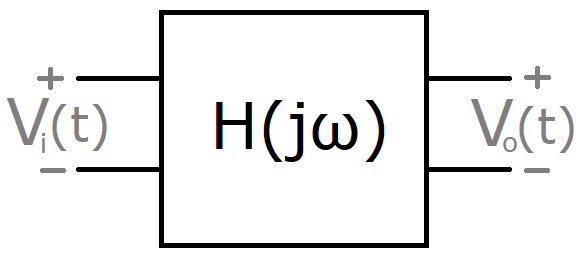
\includegraphics[width=10cm]{figures/signalInOutBox.png}
\caption{A generic frequency-dependent circuit with an input and an output voltage.}
\label{inOutSignalBox}
\end{figure}

This box takes a voltage signal $v_i(t)$ as its input and presents a voltage signal $v_o(t)$ at its output terminals. The output voltage, $V_o(t)$ is related to $V_i(t)$ by H($j\omega$), which is known as the \textbf{frequency response} of the system in the box. Note that frequency response is not a function of time, but frequency. In general, for any system with an input voltage and an output voltage, the definition for frequency response is
$$
\mathnormal{H(j\omega)} = \frac{V_o}{V_i}
$$
Where $V_o$ and $V_i$ represent the phasor forms for these voltages. 
\par
Before we get into specifics, let's look at the circuit of Figure \ref{voltageDivWithBoxElements}. We have very limited information here, but we can still express the frequency response of the circuit in terms of the impedances given. 
\begin{figure}[h!]
\centering
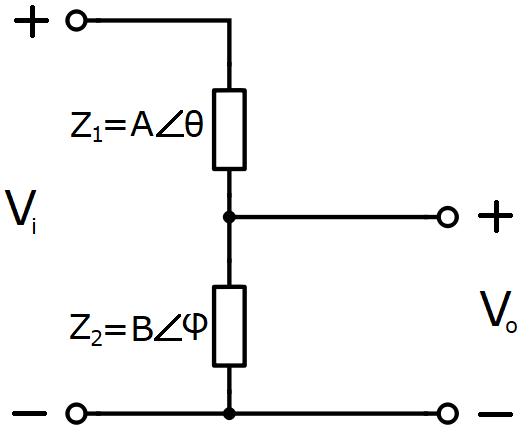
\includegraphics[width=10cm]{figures/voltageDivBoxes.png}
\caption{A generic voltage divider comprised of two sections of elements each with their own impedance.}
\label{voltageDivWithBoxElements}
\end{figure}
Using the voltage divider rule, we know how to relate the voltage across Z$_2$ ($V_o$) to the input voltage $V_i$:
$$
V_o = V_i\cdot\left(\frac{Z_2}{Z_1+Z_2}\right)
$$
We aren't interested in an exact value for $V_o$, but we can use this expression to find the frequency response for the circuit by dividing both sides by $V_i$:
$$
H(j\omega) = \left(\frac{Z_2}{Z_1+Z_2}\right)
$$
If we had specific values for these impedances, we could analyze the resulting frequency response to determine the filtering behavior for the circuit. In the following sections, we will do this analysis with several common passive filters that use just resistors, capacitors, and inductors.

\section{RC High-Pass and Low-Pass Filters}
Consider the circuit of Figure \ref{RC_HP}. This is just a voltage divider with a resistor and a capacitor, and the output of the circuit is the voltage across the resistor. 
\begin{figure}[h!]
\centering
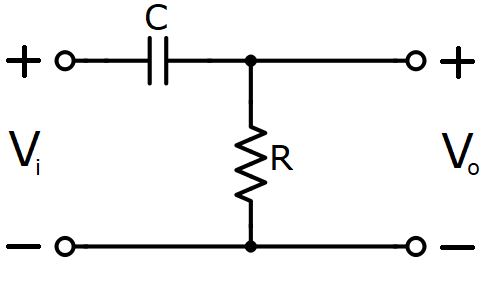
\includegraphics[width=10cm]{figures/RC_HP.png}
\caption{A voltage divider with a resistor and a capacitor.}
\label{RC_HP}
\end{figure}
As we did before, we can determine the frequency response for this system by using the voltage divider rule:
$$
H(j\omega) = \frac{Z_R}{Z_R+Z_C} = \frac{R}{R+(1/j\omega C)}
$$
This is a function of frequency like we want, but its current form is gross. We need to make it look better so we can more easily analyze the behavior of the system. One way to improve it is to get rid of the fraction in the denominator. To do this, we will multiply both the numerator and the denominator by $j\omega C$:\footnote{I call this process ``multiplying by a fancy 1'', because we are really just multiplying the whole frequency response by 1, but it's a form of 1 that works to our advantage.}
$$
H(j\omega) = \frac{R}{R+(1/j\omega C)}\cdot\frac{j\omega C}{j\omega C}
$$
$$
= \frac{j\omega RC}{j\omega RC +1}
$$
\par
This is a much more satisfying form of the frequency response for this circuit. Now that we have determined the frequency response, let's analyze the behavior of this circuit at different driving frequencies. Of course, there is an infinite range of frequencies, but we can get a sense of the behavior of a circuit by determining what happens to the frequency response at $\omega=0$ and as $\omega\rightarrow\infty$:
$$
\textnormal{For }\omega=0\textnormal{: }H(0) = \frac{0}{1} = 0
$$
$$
\textnormal{For }\omega\rightarrow\infty\textnormal{: }H(j\infty) = \frac{j\infty}{j\infty+1} \approx 1
$$
So, for $\omega=0$, the output voltage is 0. This is akin to connecting a DC source to the input for the circuit. This tells us that the filter in question preferrentially attenuates signals of lower frequency. Conversely, as the frequency approaches infinity, the frequency response approaches 1, which means that the output voltage is equal to the input voltage. These two conditions for the frequency response tell us that this circuit is a \textbf{high-pass filter}, because it allows signals of high frequency to pass through unchanged, while lower frequencies are attenuated.
\begin{figure}[h!]
\centering
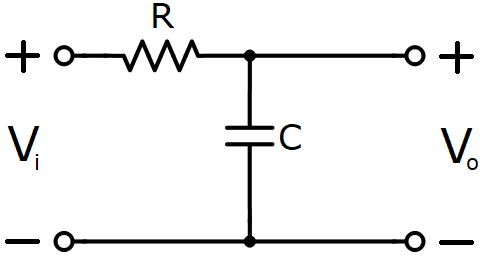
\includegraphics[width=10cm]{figures/RC_LP.png}
\caption{Another voltage divider with a resistor and a capacitor.}
\label{RC_LP}
\end{figure}
\par
Now let's analyze the circuit of Figure \ref{RC_LP}. This is a voltage divider with just a resistor and capacitor, too, but in this system we are taking the output $V_o$ from across the capacitor. This results in the following frequency response:
$$
H(j\omega) = \frac{Z_C}{Z_R+Z_C} = \frac{\frac{1}{j\omega C}}{R+(1/j\omega C)}
$$
Again, we will get rid of the fractions in the numerator and denominator of this expression by multiplying both by $j\omega C$:
$$
H(j\omega) = \frac{\frac{1}{j\omega C}}{R+(1/j\omega C)}\cdot\frac{j\omega C}{j\omega C} 
$$
$$
= \frac{1}{j\omega RC + 1}
$$
\par
Now let's consider the frequency response for the cases we considered before. If $\omega=0$, H(j0)=1. This tells us that when the frequency of the input signal is low, the output is roughly equal to the input. However, when $\omega\rightarrow\infty$, H(j$\infty$)$\approx$ 0. This means that as the frequency of the input signal increases, the amplitude of the output voltage decreases. We call this circuit a \textbf{low-pass filter}, because if the input signal frequency is low, it will be allowed to pass through the filter without its amplitude decreasing.
\par
For both of these types of filters, it would be nice to have a way to quantify their frequency responses without simply citing a frequency-dependent function. Fortunately, we can describe their behavior in terms of a single \textbf{cutoff frequency}, $\omega_c$. This is defined as follows:
$$
|H(j\omega_c)| = \frac{1}{\sqrt{2}}
$$
Why $\sqrt{2}$? Remember the form of Watt's law that says power delivered to an element is proportional to the voltage across that element squared? Well, if the frequency response of one of these filters is equal to $\frac{1}{\sqrt{2}}$, that means the output voltage can deliver just half the amount of power to a load that could have been delivered by the input voltage. Because of this, the cutoff frequency is also called the \textbf{half-power frequency}. Below, I derive the definition of the cutoff frequency using the frequency response of the low-pass filter:
$$
\frac{1}{\sqrt{2}} = |H(j\omega_c)| = \left|\frac{1}{j\omega_c RC +1}\right|
$$
$$
\sqrt{2} = |(j\omega_c RC +1)| = \sqrt{(1 + j\omega_c RC)\cdot(1 - j\omega_c RC)}
$$
$$
= \sqrt{(1 \cancel{+ j\omega_c RC - j\omega_c RC} - \cancelto{-1}{j^2}\omega_c^2(RC)^2)} = \sqrt{1+ \omega_c^2 (RC)^2}
$$
$$
2 = 1+\omega_c^2(RC)^2
$$
$$
\frac{1}{(RC)^2}=\omega_c^2
$$
$$
\omega_c=\frac{1}{RC}
$$
While we derived this definition using the frequency response for the low-pass filter, both high-pass and low-pass filter types have the same definition for cutoff frequency. When describing a filter circuit in practice, we will usually give a cutoff frequency and a filter type rather than citing the full frequency response expression.


%Both the high-pass and the low-pass filters are just voltage dividers comprised of a single resistor in series with a single capacitor. The main difference between these two filters is the element across which the output voltage is measured. 
%\par 
%Let's add the frequency responses for both of these filters together; I'll use subscripts ``HP'' and ``LP'' to distinguish between the frequency response of the high-pass filter and low-pass filter, respectively:
%$$
%H_{HP}(j\omega) + H_{LP}(j\omega) = \frac{j\omega RC}{j\omega RC +1} + \frac{1}{j\omega RC + 1} = \frac{j\omega RC + 1}{j\omega RC + 1} = 1
%$$
%The fact that the sum of the two frequency responses for these systems is 1 tells us that their respective outputs are complimentary; if we drove both circuits with the same input signal, we could reproduce the input signal by summing the output signals from both systems. 

\section{RLC Band-Pass and Band-Stop Filters}
High- and low-pass filters are the most commonly seen passive filter circuits in practice. Sometimes a circuit is needed that will either allow just a single frequency to pass through, or cut a single frequency out of the input. To accomplish these tasks, a \textbf{Band-Pass} or a \textbf{Band-Stop} Filter, respectively, could be used.
\begin{figure}[h!]
\centering
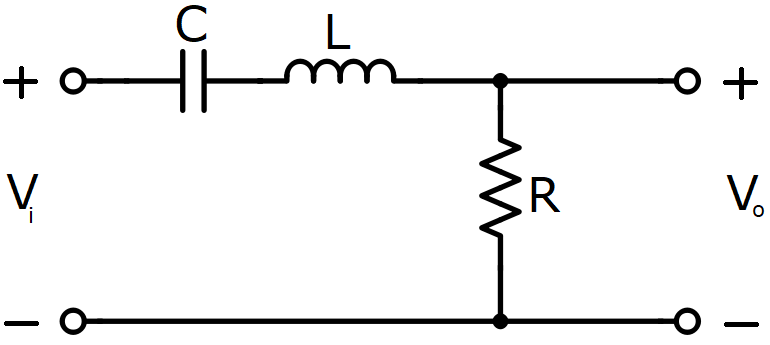
\includegraphics[width=10cm]{figures/BPfilter.png}
\caption{A voltage divider comprised of a capacitor, inductor, and resistor.}
\label{RLC_BP}
\end{figure}
\par
Consider the circuit in Figure \ref{RLC_BP}. This circuit is a voltage divider comprised of a capacitor, an inductor, and a resistor. We can again define $H(j\omega)$ using the voltage divider rule as follows:
$$
H(j\omega) = \frac{Z_R}{Z_R+Z_L+Z_C} = \frac{R}{R + j\omega L+\frac{1}{j\omega C}} = \frac{R}{R + j\left(\omega L-\frac{1}{\omega C}\right)}
$$
This frequency response differs from those of the high- and low- pass filters in one major way---its imaginary component is the difference of two frequency-dependent terms. This means that there is a particular input frequency (which we will call the \textbf{resonant frequency} for the circuit, $\omega_0$) that will cause those two terms to cancel each other. If that were the case, the amplitude of the frequency response would be 
$$
\left|H(j\omega_0)\right|=\left|\frac{R}{R + j\cancelto{0}{\left(\omega_0\cdot L-\frac{1}{\omega_0\cdot C}\right)}}\right| = 1
$$
This demonstrates that at that particular frequency, the input would pass through to the output without losing any amplitude. 
\par
Now let's determine what would happen at the two extreme ends of the valid frequency range. If the frequency were 0, the amplitude of the frequency response would be
$$
\left|H(j\cdot0)\right|=\left|\frac{R}{R + j\left(0\cdot L-\cancelto{\infty}{\frac{1}{0\cdot C}}\right)}\right| = 0 
$$
If instead, the frequency approaches infinity, the frequency response would be
$$
\left|H(j\cdot\infty)\right|=\left|\frac{R}{R + j\left(\infty\cdot L-\cancelto{0}{\frac{1}{\infty\cdot C}}\right)}\right| = 0 
$$
In both of these cases, the output amplitude is diminished to 0. We can extrapolate these three cases to conclude that this filter only allows some frequencies close to the resonant frequency, $\omega_0$, to pass through to the output, and the rest of the frequency range is attenuated (i.e., cut out). This circuit is called a \textbf{Band-Pass Filter}, because it only allows a ``band'' of frequencies to pass through from input to output. 
\par
A band-pass filter can, of course, be characterized with its frequency response formula, but in practice we use its resonant frequency and its \textbf{bandwidth} to describe its behavior. To determine its resonant frequency, we set the imaginary component to zero and then solve that equation for $\omega_0$:
$$
\omega_0 L-\frac{1}{\omega_0 C} = 0
$$
$$
\omega_0 L = \frac{1}{\omega_0 C}
$$
$$
\omega_0^2 = \frac{1}{LC}
$$
$$
\omega_0 = \frac{1}{\sqrt{LC}}
$$
The next quantity we want to determine is the \textbf{bandwidth} of the circuit. The bandwidth is a measure of how dramatically the output of the filter attenuates as the input frequency is swept off of the resonant frequency. We call this the ``bandwidth'' because it is the actual width (in dimensions of frequency) of the band of frequencies that are passed through the circuit. Quantitatively, the bandwidth of a band-pass filter is simply the difference between its two half-power frequencies. We found the half-power frequency for the high-pass and low-pass filters in the last section, but each of those filters only had single half-power frequency. The band-pass filter has two such frequencies. I will not derive them here, because it requires a tedious calculation, and nobody wants that\footnote{If you do want to see this derivation, you can find it online, or better yet, do it yourself! But be prepared with the quadratic formula and lots of paper.}. The \textbf{bandwidth} for the filter is
$$
\beta = \frac{R}{L}
$$
\par
This expression for the bandwidth tells us that if the resistor in the filter is of a high value, the pass-band of frequencies is wide, whereas if the resistance is small, the pass-band is narrow. Note that the bandwidth is not dependent on the value of the capacitor.
\par
The last type of filter I will introduce in this chapter is the \textbf{Band-Stop Filter}. Its general form is shown in Figure \ref{RLC_BS}. 
\begin{figure}[h!]
\centering
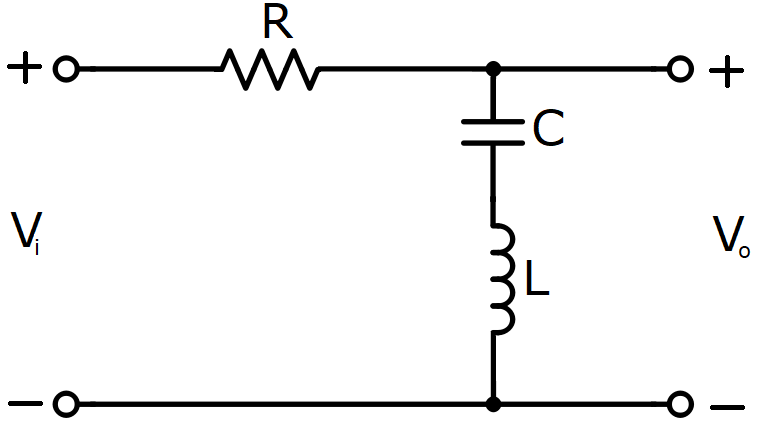
\includegraphics[width=10cm]{figures/BSfilter.png}
\caption{Another voltage divider comprised of a capacitor, inductor, and resistor.}
\label{RLC_BS}
\end{figure}
Does this circuit look familiar? Hopefully by now you have noticed that all our filters are really just voltage dividers. I told you those were useful!
\par
The band-stop filter is just like the band-pass filter, except that instead of measuring the output voltage across the resistor, we now measure $V_o$ across the capacitor and inductor together. The frequency response for this filter is
$$
H(j\omega) = \frac{Z_L+Z_C}{Z_R+Z_L+Z_C} = \frac{j\omega L+\frac{1}{j\omega C}}{R + j\omega L+\frac{1}{j\omega C}} = \frac{j\left(\omega L-\frac{1}{\omega C}\right)}{R + j\left(\omega L-\frac{1}{\omega C}\right)}
$$
\par
Like the band-pass filter, the band-stop filter has a resonant frequency and a bandwidth:
$$
\omega_0 = \frac{1}{\sqrt{LC}}
$$
$$
\beta = \frac{R}{L}
$$
The behavior of the band-stop filter is opposite that of the band-pass filter, however; instead of only allowing a small band of frequencies to pass through the filter, the band-stop filter \textit{stops} a band of frequencies from passing through. Yes, the name says it all.

\section{Limitations of Passive Filters}
Passive filters could not be simpler. They do have draw-backs, though. One is that the amplitude of their frequency response is at most 1, which means that a passive filter cannot make the output signal bigger in amplitude than the input signal; these filters only attenuate---they never amplify.
\par
Another limitation of these filters is that they are voltage dividers, and are affected greatly by whatever load they are connected to down-stream. However, we will learn how to mitigate this effect in the next two chapters. 
\section{Recap: Passive Filters}
Hopefully this chapter showed you that the material we have covered so far is not just theoretically interesting, but that it can be used to do something constructive. We will continue in that vein over the course of the next two chapters. For now, here is a brief synopsis of the highlights from this chapter:
\begin{description}
\item[Signal:] A time-dependent voltage or current that carries some information.
\item[Frequency Content/Frequency Spectrum:] All of the different frequencies that are contained in a signal.
\item[Filtering:] Adjusting the amplitude of a certain range of frequencies contained within a signal.
\item[Attenuation:] A decrease in amplitude. 
\item[Frequency Response:] A complex function of frequency, defined as the ratio of output voltage to input voltage for a given system:
$$
\mathnormal{H(j\omega)} = \frac{V_o}{V_i}
$$
\item[High-Pass and Low-Pass Filters:] Voltage dividers comprised of a resistor and a capacitor. The high-pass filter measures output voltage across the resistor, and it only passes input frequencies through to the output if those frequencies are greater than the cutoff frequency. The low-pass filter measures output across the capacitor, and it only passes input frequencies through to the output if those frequencies are less than the cutoff frequency.
\par
Cutoff frequency: $\omega_c = \frac{1}{RC}$
\item[Band-Pass and Band-Stop Filters:] These pass a band of frequencies from input to output, or stop a band of frequencies from progressing through the circuit to its output.
\par
Resonant frequency:  $\omega_0 = \frac{1}{\sqrt{LC}}$
\par
Bandwidth:  $\beta = \frac{R}{L}$
\end{description}
\chapter{Introduction to Operational Amplifiers}
One of the major functions of circuits is to amplify signals. This means that the output amplitude is made greater than the input amplitude. To borrow the language of the last chapter, amplification would make the frequency response of such a system greater than 1, which we saw could not happen with passive circuits involving just capacitors, inductors, and resistors. In this chapter, we will introduce a ubiquitous electronic device called the \textbf{operational amplifier} (or \textbf{op amp} for short), which is capable of amplification, filtering, and more. Most circuits today have at least one op amp, and after you read this chapter you will be able to determine what they do in the context of a larger circuit.
\section{Ideal Op Amps}
Figure \ref{firstOpAmp} shows the schematic representation of an op amp by itself. This triangle-shaped symbol obscures the guts of the device, merely showing us its most important externally-accessible nodes. There are so many different implementations of op amps available from electronic suppliers that you might think they all have vastly different characteristics. However, all op amps increase or otherwise change the amplitude of an input voltage signal and they all ideally adhere to the same rules.
\begin{figure}[h!]
\centering
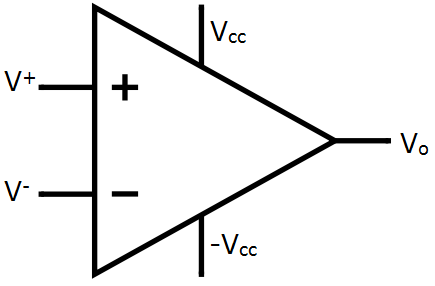
\includegraphics[width=6cm]{figures/loneOpAmp.png}
\caption{The schematic representation of an op amp.}
\label{firstOpAmp}
\end{figure}
\par
Back to the Figure \ref{firstOpAmp}: The two ports on the left are labeled with a ``+'' and a ``-''. These are referred to as the ``non-inverting'' and ``inverting'' inputs, respectively. The input voltage for our amplifier is connected to these inputs, as we will see in the next section. The port at the right of the op amp is where the output for the amplifier comes from. The two ports at the top and bottom of the amplifier are where the power supply for the op amp is connected. Most op amps require two voltage supplies---one that provides a positive voltage and another that provides a negative voltage of equal amplitude.
\par
Now that we know what all those connections are for, let's look at the simplest behavior of this device. When a voltage difference is presented across the input terminals (in other words, if $(V_+-V_-)\neq0$ in Figure \ref{firstOpAmp}), the output voltage is linearly proportional to that input:
$$
V_o = A_{ol}\cdot (V_+-V_-)
$$
In this expression, $A_{ol}$ is the \textbf{open-loop gain} for the op amp, and typical values for $A_{ol}$ are $\sim10^5$. This is extremely large! If the power supply for the op amp allowed it, in this configuration even a very modest input voltage amplitude of 1mV would produce an output voltage amplitude of 100V! In practice, the amplitude of a signal in this configuration is limited by the positive and negative voltage supplies for the op amp (V$_{\textnormal{cc}}$ and -V$_{\textnormal{cc}}$ in Figure \ref{firstOpAmp}); the output voltage of an op amp cannot exceed the positive or negative supply voltages, and if its amplitude would ever exceed those limits, it will be ``clipped'' at the op amp power supply voltages. However, the open-loop gain is an internal property of an op amp that is based on its fabrication parameters and which we cannot change. So, in this configuration, an op amp isn't really very useful. We need a way to ``reign in'' the gain of this device.
\par
Op amps are really useful when we connect their output voltage back to their inverting input in some way. This is called \textbf{negative feedback}, and it is called this because we feed the output back to the negative input. Makes sense, right? When op amps are configured with negative feedback, they obey two rules that we will use to analyze their behavior:
\begin{enumerate}
\item No current flows into or out of the inverting or non-inverting input
\item There is no voltage difference between the input terminals (you can treat the inverting and non-inverting inputs as the same node)
\end{enumerate}
In the next several sections, we will analyze some common configurations of resistive amplifier circuits using the two rules above.
\section{Unity Gain Buffer}
The simplest op amp configuration with negative feedback is known as a \textbf{unity gain buffer}, and its schematic is shown in Figure \ref{unityGainBuffer}.
\begin{figure}[h!]
\centering
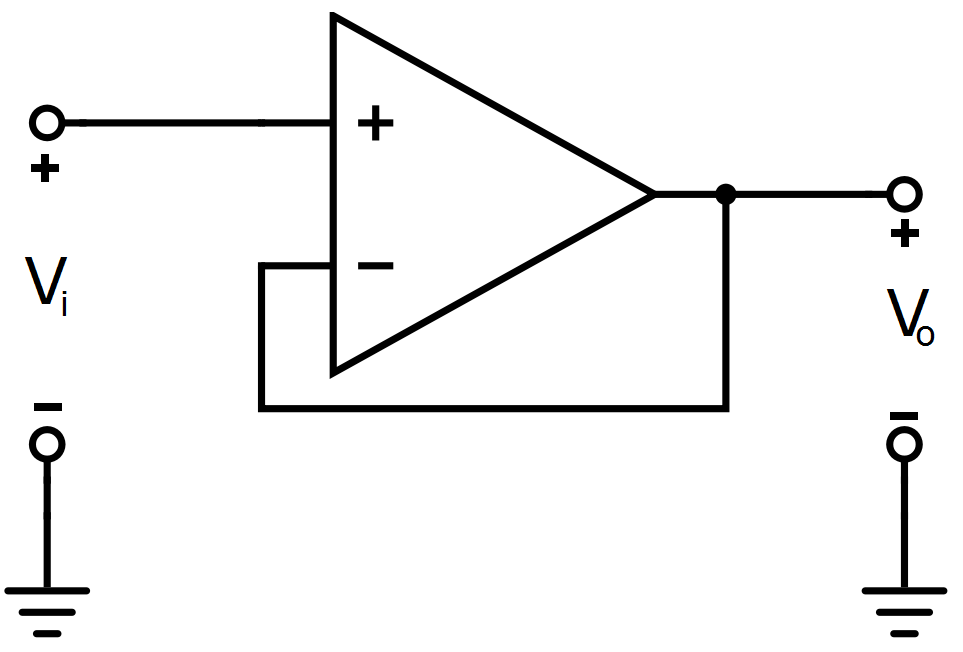
\includegraphics[width=7cm]{figures/unityGainBuffer.png}
\caption{An op amp in the unity gain buffer configuration.}
\label{unityGainBuffer}
\end{figure}
Using the rule that there is no voltage difference between the input terminals of the op amp, we can easily determine that $V_o=V_i$. Why would anyone use one of these? Well, even though we didn't change the input \textit{voltage}, the op amp can ideally drive any load without being affected by that load. Remember when we talked about voltage dividers being loaded down? If we connect a unity gain buffer to the output of a voltage divider, the op amp can then ideally drive any load without that load affecting the voltage. We will revisit this configuration in the next chapter.

\section{Inverting Amplifier}
\begin{figure}[h!]
\centering
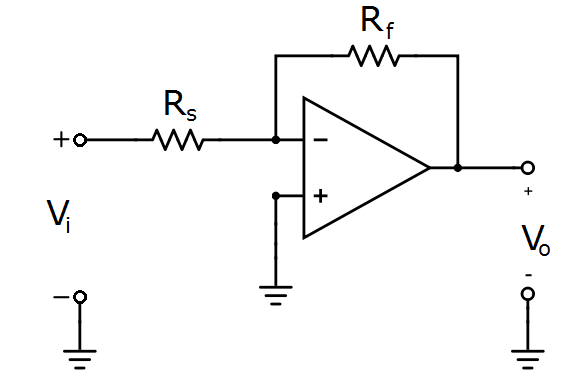
\includegraphics[width=7cm]{figures/invertingAmplifier.png}
\caption{An inverting amplifier op amp configuration.}
\label{invertingAmplifier}
\end{figure}
Let's look at the circuit of Figure \ref{invertingAmplifier}. Note that in this circuit, we have omitted the voltage supply inputs for the op amp. This is common practice when analyzing op amp configurations because it removes unnecessary clutter from the diagram. This circuit incorporates negative feedback through a resistor, $R_f$. Because this circuit has negative feedback, we can use two ideal op amp rules from the last section to determine an expression for the output voltage.
\par
Let's use the second rule of our two op amp rules to declare the inverting input node to be grounded. We can do this because the non-inverting input is grounded, and the second rule states that there is no voltage difference between the two inputs. Therefore, the circuit can be reduced to that shown in Figure \ref{invertingAmplifier2}, where the inverting input is now grounded. 
\begin{figure}[h!]
\centering
\includegraphics[width=7cm]{figures/invertingAmplifier2.png}
\caption{An inverting amplifier op amp configuration, with both the inputs explicitly grounded.}
\label{invertingAmplifier2}
\end{figure}
\par
Next, taking into account the fact that there is no current flowing into the inverting input allows us to completely remove the op amp as shown in Figure \ref{invertingAmplifier3}. Now we just have to solve for $V_o$ in terms of $V_i$ using the techniques we learned all the way back in Chapter \ref{chap:resistorRulesAndTricks}, because all that remains of our original circuit is a resistor network. I have also labeled this figure with currents $i_s$ and $i_f$ which will be helpful in our analysis.
\begin{figure}[h!]
\centering
\includegraphics[width=7cm]{figures/invertingAmplifier3.png}
\caption{An inverting amplifier op amp configuration with the op amp removed!}
\label{invertingAmplifier3}
\end{figure}
\par
Let's start by determining how those currents are defined. We can see that according to KVL, the voltage across $R_s$ is $V_i$. Also, according to Ohm's law, $V_i = i_s\cdot R_s$, so $i_s = V_i/R_s$. Next, let's find a definition for $i_f$; by the same logic as before, $V_o = i_f\cdot R_f$, therefore $i_f = V_o/R_f$.
\par
Knowing the definitions for these currents is fine, but we don't want them in our final expression for $V_o$. Notice that at the node between the two resistors in Figure \ref{invertingAmplifier3}, there is a current coming in from the left and a current coming in from the right, but there doesn't appear to be a current flowing out of the node. According to KCL, the current flowing in should be equal to the current flowing out, but if there is no current flowing out, 
$$
i_s + i_f = 0
$$
This means that one of these currents must be negative. That may not seem possible, but a negative current is just a current whose arrow is pointed in the opposite direction from how it actually flows. Let's plug our expressions for these currents into this expression, and then finally solve for $V_o$:
$$
\frac{V_i}{R_s} + \frac{V_o}{R_f} = 0
$$
$$
\frac{V_o}{R_f} = -\frac{V_i}{R_s}
$$
$$
V_o = -\frac{R_f}{R_s}V_i
$$
\par
This expression shows us that the output voltage is a negated version of the input voltage. This amplifier configuration is known as an \textbf{inverting amplifier}, because the output voltage is \textit{inverted} (i.e., negative) with respect to the input voltage. Additionally, the output is scaled by a factor of $R_f/R_s$; these resistors can be chosen so that the scaling factor can have any value we want.
\par
All amplifier systems can be characterized by their \textbf{gain}, and for op amps, we most often refer to \textbf{voltage gain}, which is defined as 
$$
A_V = \frac{V_o}{V_i}
$$
Sometimes $A_V$ is a function of frequency, but for the amplifier of Figure \ref{invertingAmplifier}, the voltage gain is defined as
$$
A_V = -\left(\frac{R_f}{R_s}\right)
$$
Inverting amplifiers are characterized by their negative gain, and you can recognize them schematically by the fact that their input voltage is connected to their inverting input.
\section{Non-Inverting Amplifier}
\begin{figure}[h!]
\centering
\includegraphics[width=7cm]{figures/nonInvertingAmp.png}
\caption{A non-inverting amplifier circuit.}
\label{nonInvertingAmp}
\end{figure}
Now let's look at the circuit of Figure \ref{nonInvertingAmp}. This circuit has negative feedback, so we can again use the two ideal op amp rules to determine the voltage gain for this amplifier configuration.
\par
The voltage with respect to ground at the non-inverting input to the op amp is $V_i$. Because there is no voltage difference between the inverting and non-inverting inputs for the op amp, we can treat the inverting input voltage as $V_i$, too. Furthermore, given the fact that there is no current flowing into the inputs of the op amp, we can re-draw the circuit without the op amp as shown in Figure \ref{nonInvertingSansAmp}.
\begin{figure}[h!]
\centering
\includegraphics[width=7cm]{figures/nonInvertingSansAmp.png}
\caption{A non-inverting amplifier circuit with the op amp removed.}
\label{nonInvertingSansAmp}
\end{figure}
\par
From this figure, you can see that the resistors make a voltage divider. This voltage divider looks a little strange, however, since $V_i$ is the smaller of the two voltages in this configuration. Nevertheless, we can use the voltage divider rule to relate the input and output voltages:
$$
V_i = V_o\left(\frac{R_g}{R_f+R_g}\right)
$$
Using this expression, we can solve for voltage gain:
$$
A_V = \frac{V_o}{V_i} = \frac{R_f+R_g}{R_g} = 1 + \frac{R_f}{R_g}
$$
This type of amplifier configuration is known as a \textbf{non-inverting amplifier}, because its gain is not inverted. Note that its voltage gain is always at least 1.

\section{Summing Amplifier}
The circuit in Figure \ref{summingAmp} is another common amplifier configuration called a \textbf{non-inverting summing amplifier}. 
\begin{figure}[h!]
\centering
\includegraphics[width=10cm]{figures/nonInvertingSummingAmp.png}
\caption{A summing amplifier circuit.}
\label{summingAmp}
\end{figure}
This circuit has more pieces than the other two configurations we have already looked at, but we can determine its voltage gain in the same way as before. First, we can solve for the inverting input voltage using the voltage divider rule:
$$
V_- = V_o\left(\frac{R_g}{R_g+R_f}\right)
$$
Next, we need to determine the voltage of the non-inverting input. To do so, we will use the fact that only one current can flow between $V_i1$ and $V_i2$, since no current flows into the op amp. Let's call that current $i_{12}$, and let's assume it travels from input $V_i1$ to $V_i2$. We can use this current to deduce a KVL equation for that portion of the circuit, which will ultimately allow us to find an expression for $V_+$:
$$
V_{i1}-i_{12}\cdot R_1 = V_+
$$
We will need one additional equation to eliminate $i_{12}$ from our calculation:
$$
V_{i1}-i_{12}\cdot R_1 - i_{12}\cdot R_2 = V_{i2}
$$
Putting these all together yields
$$
V_- = V_+
$$
$$
V_o\left(\frac{R_g}{R_g+R_f}\right) = V_{i1}-i_{12}\cdot R_1
$$
$$
i_{12} = \frac{V_{i1}-V_{i2}}{R_1 + R_2}
$$
$$
V_o\left(\frac{R_g}{R_g+R_f}\right) = V_{i1}-\frac{V_{i1}-V_{i2}}{R_1 + R_2}\cdot R_1 = \frac{V_{i1}(R_1+R_2)-V_{i1}R_1+V_{i2}R_1}{R_1+R_2}
$$
$$
= \frac{\cancel{V_{i1}R_1}+V_{i1}R_2\cancel{-V_{i1}R_1}+V_{i2}R_1}{R_1+R_2}
$$
And finally, 
$$
V_o = \left(\frac{R_g+R_f}{R_g}\right)\cdot\left( \frac{V_{i1}R_2+V_{i2}R_1}{R_1+R_2}\right)
$$
\par
This is called a summing amplifier for the obvious reason that its output is a weighted sum of the input voltages. There are, of course, several resistors mixed in there, too, but assuming all of the resistors are the same value, 
$$
V_o = \left(\frac{\cancel{2R}}{\cancel{R}}\right)\cdot\left( \frac{V_{i1}\cancel{R}+V_{i2}\cancel{R}}{\cancel{2R}}\right) = V_{i1}+V_{i2}
$$
We could also add more voltages with this same configuration as long as we connect them to the non-inverting input through a resistor. Obviously, it is hard to express the gain of this amplifier configuration in the same way as the previous configurations, since there are multiple input voltages.

\section{Recap: Ideal Op Amp Rules and Resistive Amplifier Configurations}
In this chapter we covered the rules we use for analyzing op amps in circuits. We also looked at a few common configurations for resistive op amp circuits. We will be revisiting some of these in the next chapter, but with capacitors mixed in among the resistive elements. The techniques we used to find the voltage gain and expressions for $V_o$ for the circuits in this chapter apply to the analysis of any op amp circuit. Here is a brief synopsis of the main concepts of this chapter:
\begin{description}
\item[Open-Loop Configuration] This is the case when the output of an op amp is not fed back to the inverting input. The op amp then amplifies any voltage difference between the non-inverting and inverting input terminals to produce its output. The open-loop gain for an op amp is $\sim10^5$, which means even tiny input voltages are amplified to an extreme degree. This configuration has limited uses.
\item[Negative Feedback] happens when the output of an op amp is fed back into its inverting input. This allows us to design circuits with a particular value for the voltage gain as opposed to the open-loop gain.
\item[Ideal Op Amp Rules] are the two rules we assume are true for any op amp in a configuration with negative feedback:
\begin{enumerate}
\item The voltage at the inverting input is the same as the voltage at the non-inverting input
\item No current flows into the inputs of the op amp
\end{enumerate}
With these two rules, we were able to dramatically reduce the complexity of analysis.
\item[Voltage Gain] is defined as 
$$
A_V = \frac{V_o}{V_i}
$$
This is reminiscent of the frequency response of a filter, except that the voltage gain can have a value greater than 1. So far, we have only seen frequency-independent voltage gain, but in the next chapter that will change.
\item[Unity Gain Buffer] This op amp configuration produces an output voltage that is the same as the input voltage; in other words, the voltage gain of this configuration is 1. This configuration is useful for driving loads downstream in the signal path of a circuit.
\item[Inverting Amplifier] This is an amp whose output is negated with respect to its input voltage.
\item[Non-Inverting Amplifier] This is an amplifier whose output is not negated with respect to its input. 
\item[Non-Inverting Summing Amplifier]This configuration takes two or more voltages as inputs and its output is a weighted sum of those inputs. If all the resistors in the circuit are the same, however, the output is just the sum of the inputs.
\end{description}

There are several more resistive configurations for op amps, but in the next chapter we will look at similar circuits to those we saw in this chapter, except with capacitors \textit{and} resistors.
\chapter{Filters and Op Amps}
In the last chapter, we learned what op amps are and how we can use two simple rules to analyze their behavior in the context of a given circuit. In the chapter before that, we learned about passive filtering circuits, which selectively attenuate voltage signals based on their frequency content. In this chapter, we will put those concepts together to learn about \textit{active filters}, which not only attenuate signals based on frequency, but also have the potential to \text{amplify} signals in a frequency-dependent way.
\section{Passive Filters with Unity Gain Buffers}
\begin{figure}[h!]
\centering
\includegraphics[width=10cm]{figures/bufferedLP.png}
\caption{A passive low-pass filter connected to a unity gain buffer.}
\label{bufferedLP}
\end{figure}

Placing a unity gain buffer after a passive filter as shown in Figure \ref{bufferedLP} mitigates some of the shortcomings of passive filters alone. This circuit acts as a low pass filter, as is clear from the passive low pass filter connected to the non-inverting input. That input is then passed through a unity gain buffer, which can drive any load without its frequency response changing. This is great, because it has the same frequency response as the passive filter alone, and it cannot be loaded down. This configuration could be improved further if we add resistors to the feedback network, thereby providing amplification along with filtering. 
\par
However, this system does have disadvantages; since the filter portion of this circuit is completely separate from the op amp portion of the circuit, the frequency response of the entire system can be affected by passive elements connected to the front end of this circuit. Fortunately, there is a better way.
\section{Active Low-Pass Filter}
\begin{figure}[h!]
\centering
\includegraphics[width=10cm]{figures/activeLP.png}
\caption{An active low-pass filter in an inverting amplifier configuration.}
\label{activeLP}
\end{figure}
Figure \ref{activeLP} shows an inverting amplifier configuration with a resistor and a capacitor in parallel in the feedback network. This is an inverting, active low-pass filter. Let's analyze its voltage gain (which is also its frequency response). First, recall that the voltage gain of the inverting amp is given by $-\frac{Z_f}{Z_s}$. Therefore, we can find the voltage gain of this circuit if we just determine the equivalent impedances of the feedback elements and the source resistance:
$$
Z_f = \frac{1}{\frac{1}{R_f}+j\omega C_f}=\frac{R_f}{1+j\omega R_fC_f}
$$
$$
Z_s = R_s
$$
$$
A_V(j \omega) = -\left(\frac{Z_f}{Z_s}\right) = -\left(\frac{\frac{R_f}{1+j\omega R_fC_f}}{R_s}\right) = -\left(\frac{R_f}{R_s}\right)\cdot\left(\frac{1}{1+j\omega R_fC_f}\right)
$$
\par
This votage gain is the product of two terms; the first term is frequency-independent, and it matches the gain of a purely-resistive inverting amplifier with feedback and source resistors $R_f$ and $R_s$, respectively. The second term matches the frequency response of a passive low-pass filter comprised of elements $R_f$ and $C_f$. This filter is superior to the passive filter and buffer combination of Figure \ref{bufferedLP} because its frequency response is independent of the circuit elements connected either to its input or to its output.
\section{Active High-Pass Filter}
\begin{figure}[h!]
\centering
\includegraphics[width=10cm]{figures/activeHP.png}
\caption{An active high-pass filter in an inverting amplifier configuration.}
\label{activeHP}
\end{figure}
In the last section, we replaced the feedback network of an inverting amplifier with a resistor and capacitor in parallel. In this section, we will again start with an inverting amplifier configuration, but we will replace the input network with a resistor and a capacitor in series to produce an inverting, active high-pass filter, as shown in Figure \ref{activeHP}. Let's determine its voltage gain by plugging the input and feedback impedances into the general formula for the inverting amplifier voltage gain:
$$
Z_f = R_f
$$
$$
Z_s = R_s + \frac{1}{j\omega C_s}
$$
$$
A_V(j\omega) = -\left(\frac{R_f}{R_s + \frac{1}{j\omega C_s}}\right) = -\left(\frac{j\omega R_fC_s}{j\omega C_sR_s+1}\right) 
$$
$$
= -\left(\frac{R_f}{R_s}\right)\cdot\left(\frac{j\omega C_s}{j\omega C_s+(1/R_s)}\right)
$$
\par
This voltage gain, like that for the active low-pass filter, is the product of two terms. The first term is the voltage gain for a purely resistive inverting amplifier. The second term is frequency-dependent, and it mirrors the frequency response of a passive high-pass filter. This op amp configuration provides the functionality of a high-pass filter, but with amplification as well. 
\section{Active Band-Pass Filters}
\begin{figure}[h!]
\centering
\includegraphics[width=10cm]{figures/activeBP.png}
\caption{An active band-pass filter in an inverting amplifier configuration.}
\label{activeBP}
\end{figure}
I already mentioned some of the negative characteristics of passive filters, but passive band-pass filters have an additional downside in that they require an inductor to function. Inductors tend to be bulky, and that can be a real problem if you are trying to make a circuit as small as possible. The need for inductors is eliminated in the realm of active filters, however.
\par
Let's find the voltage gain for the circuit of Figure \ref{activeBP}. This circuit combines the frequency-dependent feedback and source networks from the active low- and high-pass filters of the previous sections. As we determined before, we can use the impedances of these networks to find the expression for $A_V$ as follows:
$$
Z_f = \frac{R_f}{1+ j\omega R_fC_f}
$$
$$
Z_s = R_s + \frac{1}{j\omega C_s} = \frac{1 + j\omega R_sC_s}{j\omega C_s}
$$
$$
A_V(j\omega) = -\frac{Z_f}{Z_s} = -\frac{j\omega R_fC_s}{(1+ j\omega R_fC_f)(1 + j\omega R_sC_s)}
$$
\par
Even though it looks more complicated, this expression for voltage gain is just the product of a high-pass and a low-pass filter frequency response. The low and high cutoff frequencies are $\omega_{c,low} = \frac{1}{R_fC_f}$ and $\omega_{c,high} = \frac{1}{R_sC_s}$, respectively.
\section{Recap: Op Amp Filter Circuits}
\begin{description}
\item[Active Low-Pass Filter] This filter is described by its voltage gain, which is the product of the voltage gain for a resistive inverting amplifier and the frequency response of a passive low-pass filter:
$$
A_V(j\omega) = -\left(\frac{R_f}{R_s}\right)\cdot\left(\frac{1}{1+j\omega R_fC_f}\right)
$$
\item[Active High-Pass Filter] Like that for the inverting low-pass, the voltage gain for this filter is the product of two terms---the voltage gain for a resistive inverting amplifier, and the frequency response of a passive high-pass filter:
$$
A_V(j\omega) = -\left(\frac{R_f}{R_s}\right)\cdot\left(\frac{j\omega C_s}{j\omega C_s+(1/R_s)}\right)
$$

\item[Active Band-Pass Filter] The voltage gain for this filter is the product of a high-pass and a low-pass frequency response:
$$
A_V(j\omega) = -\frac{j\omega R_fC_s}{(1+ j\omega R_fC_f)(1 + j\omega R_sC_s)}
$$
The low and high cutoff frequencies of this filter are
$$
\omega_{c,low} = \frac{1}{R_fC_f}\textnormal{             and             } \omega_{c,high} = \frac{1}{R_sC_s}
$$
\end{description}
\end{document}